\PassOptionsToPackage{hyperfootnotes=false}{hyperref}
\documentclass[a4paper,fleqn]{cas-sc}
\DeclareUnicodeCharacter{2062}{}
\usepackage[pagewise]{lineno}
% \linenumbers

\usepackage[numbers]{natbib}
\usepackage[version=4]{mhchem}
\usepackage[capitalise]{cleveref}
\usepackage{xr}
\externaldocument[supp-]{builds/part2_supplement}
\usepackage{subcaption}
\usepackage{longtable}
\usepackage{placeins}
\usepackage{needspace}
\usepackage{mathtools}
\usepackage{tabularx}
\usepackage{makecell}
\usepackage{booktabs}
\usepackage{adjustbox}
\usepackage{xspace}
\renewcommand\cellalign{rb}
\newcolumntype{P}[1]{>{\centering\arraybackslash}p{#1}}
\usepackage{xcolor}
\usepackage{siunitx}
\usepackage{xurl}
\graphicspath{{figures/part2/}}

% Typography. cas-sc sets floats, captions, header and footer in \sffamily
% (bitmap EC sans here) and its Inconsolata check fails, leaving bitmap EC
% typewriter. Set all of them in the STIX body serif, use Type 1 Inconsolata,
% and route the class's caption makers through the caption package.
\renewcommand{\sfdefault}{\rmdefault}
\usepackage[scaled=0.95]{inconsolata}
\captionsetup{font=small,labelfont=bf,labelsep=colon,justification=justified}
\captionsetup[table]{position=top,labelsep=newline,justification=raggedright,singlelinecheck=false}
\setlength{\tabcolsep}{4pt}
\makeatletter
\ExplSyntaxOn
\cs_set_eq:NN \__make_fig_caption:nn \caption@makecaption
\cs_set_eq:NN \__make_tbl_caption:nn \caption@makecaption
\ExplSyntaxOff
\makeatother

\newcommand{\Ha}{\text{Ha}}
% Species macros shared by main.tex and supplement.tex; requires mhchem and xspace.
\newcommand{\COtwo}{\ce{CO2}\xspace}
\newcommand{\HtwoO}{\ce{H2O}\xspace}
\newcommand{\MEA}{\ce{MEA}\xspace}
\newcommand{\MEAH}{\ce{MEAH+}\xspace}
\newcommand{\MEACOO}{\ce{MEACOO-}\xspace}
\newcommand{\HCOthree}{\ce{HCO3-}\xspace}
\newcommand{\COthree}{\ce{CO3^2-}\xspace}
\newcommand{\HthreeO}{\ce{H3O+}\xspace}
\newcommand{\Hydroxide}{\ce{OH-}\xspace}
\newcommand{\Ntwo}{\ce{N2}\xspace}
\newcommand{\Otwo}{\ce{O2}\xspace}
\newcommand{\NtwoO}{\ce{N2O}\xspace}


\newcommand{\A}{\text{A}}
\newcommand{\B}{\text{B}}
\newcommand{\C}{\text{C}}
\newcommand{\D}{\text{D}}
\newcommand{\code}[1]{\texttt{#1}}
\newcommand{\liq}{\ell}
\newcommand{\vap}{v}

% Suppress the class's submission footer; journal pagination remains.
\ExplSyntaxOn
\cs_set:Npn \__first_footerline: {}
\ExplSyntaxOff

\setlength{\emergencystretch}{3em}

\begin{document}
\let\WriteBookmarks\relax
\def\floatpagepagefraction{1}
\def\textpagefraction{.001}
\shorttitle{Transfer of ePC-SAFT parameters to aqueous amines}
\shortauthors{Polley}
\title[mode=title]{\texorpdfstring{Thermodynamics of \ce{CO2}-loaded aqueous amines with ePC-SAFT. Part II: transfer to MDEA, AMP, piperazine and DEA}{Thermodynamics of CO2-loaded aqueous amines with ePC-SAFT. Part II: transfer to MDEA, AMP, piperazine and DEA}}
\author[1]{Tanner W. Polley}[orcid=0009-0008-5957-4152]
\cormark[1]
\ead{tpolley3@byu.edu}
\affiliation[1]{organization={Department of Chemical Engineering, Brigham Young University},city={Provo},state={UT},postcode={84602},country={United States}}
\cortext[cor1]{Corresponding author.}
\begin{abstract}
% P:p2-abstract-01
The shared water, carbon dioxide and inorganic-ion description established for monoethanolamine in Part I is held fixed while amine-specific parameters are estimated for methyldiethanolamine (MDEA), 2-amino-2-methyl-1-propanol (AMP), piperazine (PZ) and diethanolamine (DEA).
The same equation of state accommodates their different reaction networks, but fitted pressures retain loading- and temperature-dependent errors, and PZ species residuals remain large relative to their assumed measurement scale.
Held-out partial-pressure average absolute relative deviations (AARD) are 28.19 and 18.27\,\% for MDEA against Xiao and Ermatchkov, the latter mixing conditions inside and outside the dissociation law's measured temperature range; 42.85\,\% for AMP against Kundu; 21.94\,\% for PZ against Ermatchkov; and 79.54 and 44.17\,\% for DEA against Seo and Hong and Lal.

The data sets and fitting histories differ, so these percentages do not rank the amines.
For AMP and DEA, local conditional parameter bands are much smaller than the unfitted-pressure discrepancies; MDEA bands overlap the errors, and PZ sensitivities limit the linear approximation.
At least forty false liquid splits are detected for PZ across calibration and comparison states; a separate fit with Part I's stability penalty still has at least three, two of which the standard finite search missed.
DEA reproduces fitted integral absorption heats within 0.98\,\% AARD but predicts the wrong sign of water--DEA excess enthalpy.
The results establish the extent and limitations of amine-specific calibration under a frozen shared description, rather than uniform predictive accuracy across amine classes.
\end{abstract}
\begin{keywords}
ePC-SAFT\sep{}aqueous amines\sep{}carbon dioxide\sep{}parameter transfer\sep{}phase stability
\end{keywords}
\maketitle
\section{Introduction}\label{sec:p2-introduction}
\subsection{From the MEA benchmark to transfer across amine classes}
% P:p2-introduction-01
A shared electrolyte description is useful only to the extent that it describes observations beyond those used to estimate it.
The companion Part I develops an explicit-ion electrolyte perturbed-chain statistical associating fluid theory (ePC-SAFT) description for loaded aqueous monoethanolamine (MEA), with equilibrium, caloric and density properties calculated from a common thermodynamic potential \cite{PolleyPartI}.
Its pressure AARDs at unfitted MEA concentrations are 33.89\,\% at 15 wt\% and 44.53\,\% at 45 wt\%, despite closer agreement at the fitted concentration.
Those errors motivate a test of the shared description across other amines; they do not supply a common accuracy standard for different experimental data.

% P:p2-introduction-02
Here the water, \COtwo and inorganic-ion parameters from Part I remain fixed while only amine-specific quantities are fitted.
MDEA is a tertiary amine whose reaction network contains bicarbonate formation without amine carbamate.
AMP is a sterically hindered primary amine, DEA a secondary amine, and PZ a cyclic diamine with mono- and dicarbamate chemistry.
These choices test the common bicarbonate description both without carbamate and alongside different carbamate pathways.
One example per class cannot isolate chemical class from differences in observation coverage, species representation or fitting freedom.

\subsection{Calibration, unfitted observations and phase behavior}
% P:p2-introduction-03
Published SAFT amine models distinguish parameter estimation from predictions to different extents.
Baygi and Pahlavanzadeh fit pure and binary MEA properties and then calculate ternary solubility using ideal-activity chemical speciation \cite[Sects.~3.1--3.3]{Baygi2015}.
Nasrifar and Tafazzol also organize MEA, DEA and MDEA around pure properties, binary interactions and subsequent acid-gas comparisons, using an ideal-activity treatment rather than explicit electrolyte activity coefficients \cite[Sects.~2--6]{Nasrifar2010}.
Wangler et al. estimate MDEA ion--water interactions using osmotic data before predicting reactive ternary equilibria \cite[Sects.~6.1--6.2.1]{Wangler2018}.
The present fits instead include amine-specific reactive observations, so agreement with those observations is calibration.

% P:p2-introduction-04
In this paper, held-out observations never enter a fitting objective.
That term does not imply that the data remained unseen throughout selection of the final fit.
Previously accessed observations outside the fit and comparisons made after selecting the parameters are identified separately.
Finite searches for additional phases provide numerical evidence about the calculated liquids, while experimental pressure and property comparisons measure agreement with the named observations.
Neither form of evidence alone establishes independent validation of ion parameters or qualification for absorber design.
The results follow the properties being tested, so fitted pressures, unfitted pressures, other thermodynamic properties and phase behavior each constrain the same transfer hypothesis.

\section{Thermodynamic model and transferred parameters}\label{sec:p2-model}
\subsection{Shared terms and amine-specific chemistry}
% P:p2-model-01
The residual Helmholtz energy retains the hard-chain, dispersion, association, Debye--H\"uckel and Born contributions of Part I \cite[Sect.~2]{PolleyPartI}.
The water and \COtwo component descriptions, hydronium, hydroxide, bicarbonate and carbonate, all interactions among these six shared species, and the completed water/carbonate reaction laws are held fixed.
Table~\ref{tab:p2-origins} distinguishes independent fits, literature values, parameters estimated jointly with MEA, and assumptions.
Free interactions between an amine-specific ion and a shared species remain amine-specific parameters; freezing bicarbonate does not freeze every interaction involving bicarbonate.

% Generator: docs/scientific/latex/scripts/part2_displays.py; no model evaluation.
% Input: analyses/amp_transfer/inputs/kundu/current-declarations.toml SHA256 3085081adcf6b1d5e797a49ae6b96037cc1b5bc5191f45cff699d8546d774c55
% Input: analyses/amp_transfer/inputs/redesign/refit-306-floor-coordinates.json SHA256 b8671b1abbca5c7a406147dfad2359f1c1666887fab0b4eb67e489fc80abbe99
% Input: analyses/amp_transfer/inputs/redesign/refit-306-floor-endpoint.json SHA256 6d26e1e15c89217c7e29ce1d0772aa44285158071fdf4cc1bd0f6e7fb8fb2107
% Input: analyses/amp_transfer/notebook.qmd SHA256 a46134ecc164b9304778c6d809851a64a128dd91f932e6b898da3ce04bc9fd62
% Input: analyses/amp_transfer/results/kundu/summary.json SHA256 814f2ce5a28047c470bbcab59aadf13984e7ae034b55a4239b8e5b3058d0b55e
% Input: analyses/amp_transfer/results/refit-306/kundu-pressures.csv SHA256 561d08cf41e18d6ac277ee5e2dd207904a8885274d8d45739a0ec3f56d851cdb
% Input: analyses/amp_transfer/results/refit-306/refit-306-floor-fit.json SHA256 d7ee97cb1550d2a6969de406f09048dd4326f025a79523b7e205a5c65439233c
% Input: analyses/amp_transfer/results/refit-306/summary.json SHA256 3912f54eb7821b08e05f902d3001493b269355bea383439cada4e33fc4b4128f
% Input: analyses/amp_transfer/results/refit-306/uncertainty/prediction-bands.csv SHA256 d65f885c32fc9b391305b7e0ac76ec9f0112435455d027391c66dcd1ba7a9ff0
% Input: analyses/amp_transfer/results/refit-306/uncertainty/ranking.csv SHA256 ce80d211f43c53c9f654ec85ebdd5a91ac779a827c5e992415954cacffcab2a6
% Input: analyses/dea_transfer/inputs/runs/B-2-coordinates.json SHA256 7402f93dd3334eae251b38df951d2fdc310a730bf0045871bb83482524e75beb
% Input: analyses/dea_transfer/inputs/runs/B-2-endpoint-declarations.toml SHA256 a0e6cd9a5a7796d892130fc71f756480465898fa28cb0fc8cd371e9f4b730b72
% Input: analyses/dea_transfer/inputs/runs/B-2-endpoint-document.json SHA256 91c2384ef9f7b2a035962aafb72d97435a18a94595c5f16c64c9e2ac18785cdd
% Input: analyses/dea_transfer/notebook.qmd SHA256 c08a11c9e055d810c4b04c5c421a3ac89cf9edea895c7eb2ce3225e22368373d
% Input: analyses/dea_transfer/results/figure-values.csv SHA256 58cbb7b6e6f825b0f4fba1ef19f5393ad469e8aa42a58ece391f3b3d7af4bf2c
% Input: analyses/dea_transfer/results/fits.json SHA256 b936638b0b1f83802809bea15c003c1bbcc229b23824ce61d48ac4123b80af48
% Input: analyses/dea_transfer/results/score.json SHA256 12aa281fa03ed5d34cabbe3a09174b49da105199b15f1b16087ffa33018fd64e
% Input: analyses/dea_transfer/results/uncertainty-307/prediction-bands.csv SHA256 b59d9515e2d86b3c76eea92e97343eb5b2e28512bf4e8dd9f69e359de593f9ed
% Input: analyses/dea_transfer/results/uncertainty-307/ranking.csv SHA256 14ec3184971afe521ae4be0f1d636acd3a47067df1a01feb6068d75cf63cf155
% Input: analyses/mdea_mea_workflow/notebook.qmd SHA256 55831c2a23404765f14fbcbeb2c83eb64b7245a10730ad9ad9329b85aa1c2533
% Input: analyses/mdea_mea_workflow/results/refit-298/B1-endpoint/endpoint.json SHA256 2a5341be176829d087133a1467828f762a655f92a586eb1062a5719a58142d9d
% Input: analyses/mdea_mea_workflow/results/refit-298/B1-endpoint/fitted-replay.json SHA256 6690d0b7baf4bb3f08a9437743857d965d7a4a4fd1529d4e6f8e5d234f4059e2
% Input: analyses/mdea_mea_workflow/results/refit-298/attempts.json SHA256 40e17071831a699fe380d4ac4b1b286d5d283ad434a0e704ac2803d7d22c954f
% Input: analyses/mdea_mea_workflow/results/refit-298/pressure-comparison.csv SHA256 d2cdaf4a3bc1a2b7b9b957585a6dbaec2eff15ca56c009b862dac63a2912c22c
% Input: analyses/mea_parameter_bundle/results/selected-current-best-parameters.json SHA256 f8f64820b161377a0d97d1e4ad4f6cea764cd0558dc63231d58e2096988eef97
% Input: analyses/pz_transfer/notebook.qmd SHA256 a71c49071169b4a2795c538b22d2e59c58870489e0131cecf480d5fc98622858
% Input: analyses/pz_transfer/results/holdout-A12.csv SHA256 89f6aabc166a2663ddf7be4cfdc20821cc3ef9ef46070535644f5cd2abb66b15
% Input: analyses/pz_transfer/results/reactive-A12-record.json SHA256 3eefe76e4599050e524b9a1a8354121caae0ca30de38613359cf7e1f9edc1329
% Input: analyses/pz_transfer/results/reactive-A12-residuals.csv SHA256 3c8855bba6dfaa8ed8c8e64f7c4a160cafb77fb1d85b6858e8d5520e1469e4e4
% Input: analyses/pz_transfer/results/reactive-A12-start2-endpoint.json SHA256 c24ff09badc642d5dd312f5dc03248f2e5fa4c93e3b1d91fa69fe42120297b9e
% Input: analyses/pz_transfer/results/speciation-reactions.json SHA256 64a51633b7d56ce75a1246fe51eb6a39a1f0db1abc7d75b16b2fe13df9c125be
% Input: analyses/pz_transfer/results/uncertainty-A12/ranking.csv SHA256 f266707b75ee505bb8a5226c79e6f30037696720f859ca7d239972e6f58c71fe
% Input: analyses/solvent_specification_mdea/B1-declarations.toml SHA256 7b5fd083d83731c74624707f6e9f92bad05265c9ed19d105b25cf99dd897a042
% Input: analyses/solvent_specification_mdea/inputs/B1-coordinates.json SHA256 0bca9af202313b2bd8325ccaa37a72f32a1b326099c957c5ebf35f630506c8be
% Input: analyses/solvent_specification_mdea/notebook.qmd SHA256 227db268f1475ce3e11e4873c68e3337bf217918fa0ce0bdc11deeb25f57ff88
% Input: analyses/solvent_specification_mdea/results/adoption-302/B1/pressure.json SHA256 b81bfeb21d211d64211a2bda07b5e07af2a897f828a750f01aac6142340a7820
% Input: analyses/solvent_specification_mdea/results/retained-statistics-320.json SHA256 64393229910bf06ba614d1345e1fd2d2f675e2aba1a3a9a7eaedcd33ffd07e81
% Input: analyses/solvent_specification_mdea/results/uncertainty-307/prediction-bands.csv SHA256 96fc9352b6f30dae38805b799344404528d6e49b3b45eaa42002daa8523ac0cd
% Input: analyses/solvent_specification_mdea/results/uncertainty-307/predictions.json SHA256 8fd82d94b500a2b8985ea9979e4ceb653fbfb781dc66a3d047ee68bdec0f46ba
% Input: analyses/solvent_specification_mdea/results/uncertainty-307/ranking.csv SHA256 16b4ed6165c0cc7bad4d938567c8f8e8d88bdddb3de4eb8b53c43b372f7c8e7e
% Input: docs/scientific/latex/references.bib SHA256 7dc97086df08bf802d25d2a588158a9ad3881648729bb9a5da84741ef50acd9c
% Input: docs/scientific/latex/supplement.tex SHA256 b90143f6a0711b9a7437b4845c8a5db430f8b301ff21d8f402821b105da3d5f8
\begingroup\small\setlength{\tabcolsep}{3pt}
\begin{longtable}{@{}>{\raggedright\arraybackslash}p{0.32\linewidth}>{\raggedright\arraybackslash}p{0.36\linewidth}>{\raggedright\arraybackslash}p{0.25\linewidth}@{}}
\caption{Transferred quantities and their origins. All shared quantities remain fixed here; amine-specific interactions with shared species may be fitted.}\label{tab:p2-origins}\\
\toprule Quantity & Origin in Part I & Implication here \\ \midrule\endfirsthead
\toprule Quantity & Origin in Part I & Implication here \\ \midrule\endhead
\bottomrule\endfoot
Water segment, energy and association coefficients & Independent fit to IAPWS-95 & Fixed; not fitted to any of these amines \\
\ce{CO2} segment and energy coefficients & Gross and Sadowski, Table 2 \cite{Gross2001} & Literature inputs; fixed \\
\ce{CO2}--water dispersion correction and slope & Independent fit to Kiepe pressures & Fixed \\
Inorganic-ion segment sizes and energies & Uyan et al., Table 4 \cite{Uyan2015} & Fixed; hydrogen-ion values used for hydronium \\
Inorganic Born sizes and remaining water--ion terms & Assumed inputs in Part I & Fixed; not independently measured in MEA \\
Bicarbonate--water interaction & MEA joint fit, upper bound $+1$ & Fixed at bound; conditional SE excludes this direction \\
Completed R2 reaction level and enthalpy correction & MEA joint fit; interior with conditional errors & Fixed; source-law correction, not a new measurement \\
R1 and R3 water/carbonate laws & Literature laws as mapped in Part I & Fixed with source-reference conversion \\
Solvation and dielectric descriptions & Literature coefficients and assumptions in Part I & Water/CO2 inputs fixed; amine coefficients specified separately \\
Reactive coordinates (MDEA / AMP / PZ / DEA) & Amine-specific fits: 9 / 9 / 12 / 4 & Not totals of earlier pure and binary fitting \\
\end{longtable}\endgroup


% P:p2-model-02
Each liquid contains the shared species and its molecular amine and protonated forms.
AMP and DEA also contain carbamate; PZ contains singly and doubly protonated PZ, mono- and dicarbamate, and the neutral zwitterion HPZCOO.
The final reactive fits have nine free coordinates for MDEA, nine for AMP, twelve for PZ and four for DEA, excluding earlier pure-component, binary and dielectric fits.
Supplementary Section~S1 gives species parameters, site descriptions, diameter ties and temperature laws.
The fitted ion diameters and reaction-law corrections are effective model parameters, not independently measured molecular sizes or equilibrium constants.

% P:p2-model-03
Charged species remain liquid-only.
The vapor contains water, \COtwo and molecular amine, and for PZ also HPZCOO.
Allowing this neutral zwitterion in the vapor resolves otherwise undecided phase searches; at the earlier fixed PZ fit, the relative change in fitted partial pressures is at most $1.2\times10^{-8}$.
This numerical change is negligible for those pressures, but the vapor composition space matters to the phase search.
PZ has no solid-phase description, and its pure-liquid density is unvalidated.

\subsection{Reaction conventions and measured temperature ranges}\label{sec:p2-laws}
% P:p2-model-04
The pure-liquid solvent and infinite-dilution solute conventions follow Part I.
The amine laws and shared R2 retain their source molality standard state; R1 and R3 retain the source mole-fraction basis.
Explicit water activity and the same hydronium reference are used, with the conversions described in Part I.
For a reaction written with stoichiometric coefficients $\nu_i$ positive for products, equilibrium requires
\begin{equation}
 \sum_i\nu_i\mu_i=0,\qquad \ln K(T)=a+b/T+c\ln(T/T_0)+dT+\cdots .
 \label{eq:p2-law}
\end{equation}
Source constants are mapped to this reference once; mole-fraction and molality constants are not interchanged without their standard-state conversion.
Declared calculation intervals and measured source intervals answer different questions, as shown in Table~\ref{tab:p2-laws}.

% Generator: docs/scientific/latex/scripts/part2_displays.py; no model evaluation.
% Input: analyses/amp_transfer/inputs/kundu/current-declarations.toml SHA256 3085081adcf6b1d5e797a49ae6b96037cc1b5bc5191f45cff699d8546d774c55
% Input: analyses/amp_transfer/inputs/redesign/refit-306-floor-coordinates.json SHA256 b8671b1abbca5c7a406147dfad2359f1c1666887fab0b4eb67e489fc80abbe99
% Input: analyses/amp_transfer/inputs/redesign/refit-306-floor-endpoint.json SHA256 6d26e1e15c89217c7e29ce1d0772aa44285158071fdf4cc1bd0f6e7fb8fb2107
% Input: analyses/amp_transfer/notebook.qmd SHA256 a46134ecc164b9304778c6d809851a64a128dd91f932e6b898da3ce04bc9fd62
% Input: analyses/amp_transfer/results/kundu/summary.json SHA256 814f2ce5a28047c470bbcab59aadf13984e7ae034b55a4239b8e5b3058d0b55e
% Input: analyses/amp_transfer/results/refit-306/kundu-pressures.csv SHA256 561d08cf41e18d6ac277ee5e2dd207904a8885274d8d45739a0ec3f56d851cdb
% Input: analyses/amp_transfer/results/refit-306/refit-306-floor-fit.json SHA256 d7ee97cb1550d2a6969de406f09048dd4326f025a79523b7e205a5c65439233c
% Input: analyses/amp_transfer/results/refit-306/summary.json SHA256 3912f54eb7821b08e05f902d3001493b269355bea383439cada4e33fc4b4128f
% Input: analyses/amp_transfer/results/refit-306/uncertainty/prediction-bands.csv SHA256 d65f885c32fc9b391305b7e0ac76ec9f0112435455d027391c66dcd1ba7a9ff0
% Input: analyses/amp_transfer/results/refit-306/uncertainty/ranking.csv SHA256 ce80d211f43c53c9f654ec85ebdd5a91ac779a827c5e992415954cacffcab2a6
% Input: analyses/dea_transfer/inputs/runs/B-2-coordinates.json SHA256 7402f93dd3334eae251b38df951d2fdc310a730bf0045871bb83482524e75beb
% Input: analyses/dea_transfer/inputs/runs/B-2-endpoint-declarations.toml SHA256 a0e6cd9a5a7796d892130fc71f756480465898fa28cb0fc8cd371e9f4b730b72
% Input: analyses/dea_transfer/inputs/runs/B-2-endpoint-document.json SHA256 91c2384ef9f7b2a035962aafb72d97435a18a94595c5f16c64c9e2ac18785cdd
% Input: analyses/dea_transfer/notebook.qmd SHA256 c08a11c9e055d810c4b04c5c421a3ac89cf9edea895c7eb2ce3225e22368373d
% Input: analyses/dea_transfer/results/figure-values.csv SHA256 58cbb7b6e6f825b0f4fba1ef19f5393ad469e8aa42a58ece391f3b3d7af4bf2c
% Input: analyses/dea_transfer/results/fits.json SHA256 b936638b0b1f83802809bea15c003c1bbcc229b23824ce61d48ac4123b80af48
% Input: analyses/dea_transfer/results/score.json SHA256 12aa281fa03ed5d34cabbe3a09174b49da105199b15f1b16087ffa33018fd64e
% Input: analyses/dea_transfer/results/uncertainty-307/prediction-bands.csv SHA256 b59d9515e2d86b3c76eea92e97343eb5b2e28512bf4e8dd9f69e359de593f9ed
% Input: analyses/dea_transfer/results/uncertainty-307/ranking.csv SHA256 14ec3184971afe521ae4be0f1d636acd3a47067df1a01feb6068d75cf63cf155
% Input: analyses/mdea_mea_workflow/notebook.qmd SHA256 55831c2a23404765f14fbcbeb2c83eb64b7245a10730ad9ad9329b85aa1c2533
% Input: analyses/mdea_mea_workflow/results/refit-298/B1-endpoint/endpoint.json SHA256 2a5341be176829d087133a1467828f762a655f92a586eb1062a5719a58142d9d
% Input: analyses/mdea_mea_workflow/results/refit-298/B1-endpoint/fitted-replay.json SHA256 6690d0b7baf4bb3f08a9437743857d965d7a4a4fd1529d4e6f8e5d234f4059e2
% Input: analyses/mdea_mea_workflow/results/refit-298/attempts.json SHA256 40e17071831a699fe380d4ac4b1b286d5d283ad434a0e704ac2803d7d22c954f
% Input: analyses/mdea_mea_workflow/results/refit-298/pressure-comparison.csv SHA256 d2cdaf4a3bc1a2b7b9b957585a6dbaec2eff15ca56c009b862dac63a2912c22c
% Input: analyses/mea_parameter_bundle/results/selected-current-best-parameters.json SHA256 f8f64820b161377a0d97d1e4ad4f6cea764cd0558dc63231d58e2096988eef97
% Input: analyses/pz_transfer/notebook.qmd SHA256 a71c49071169b4a2795c538b22d2e59c58870489e0131cecf480d5fc98622858
% Input: analyses/pz_transfer/results/holdout-A12.csv SHA256 89f6aabc166a2663ddf7be4cfdc20821cc3ef9ef46070535644f5cd2abb66b15
% Input: analyses/pz_transfer/results/reactive-A12-record.json SHA256 3eefe76e4599050e524b9a1a8354121caae0ca30de38613359cf7e1f9edc1329
% Input: analyses/pz_transfer/results/reactive-A12-residuals.csv SHA256 3c8855bba6dfaa8ed8c8e64f7c4a160cafb77fb1d85b6858e8d5520e1469e4e4
% Input: analyses/pz_transfer/results/reactive-A12-start2-endpoint.json SHA256 c24ff09badc642d5dd312f5dc03248f2e5fa4c93e3b1d91fa69fe42120297b9e
% Input: analyses/pz_transfer/results/speciation-reactions.json SHA256 64a51633b7d56ce75a1246fe51eb6a39a1f0db1abc7d75b16b2fe13df9c125be
% Input: analyses/pz_transfer/results/uncertainty-A12/ranking.csv SHA256 f266707b75ee505bb8a5226c79e6f30037696720f859ca7d239972e6f58c71fe
% Input: analyses/solvent_specification_mdea/B1-declarations.toml SHA256 7b5fd083d83731c74624707f6e9f92bad05265c9ed19d105b25cf99dd897a042
% Input: analyses/solvent_specification_mdea/inputs/B1-coordinates.json SHA256 0bca9af202313b2bd8325ccaa37a72f32a1b326099c957c5ebf35f630506c8be
% Input: analyses/solvent_specification_mdea/notebook.qmd SHA256 227db268f1475ce3e11e4873c68e3337bf217918fa0ce0bdc11deeb25f57ff88
% Input: analyses/solvent_specification_mdea/results/adoption-302/B1/pressure.json SHA256 b81bfeb21d211d64211a2bda07b5e07af2a897f828a750f01aac6142340a7820
% Input: analyses/solvent_specification_mdea/results/retained-statistics-320.json SHA256 64393229910bf06ba614d1345e1fd2d2f675e2aba1a3a9a7eaedcd33ffd07e81
% Input: analyses/solvent_specification_mdea/results/uncertainty-307/prediction-bands.csv SHA256 96fc9352b6f30dae38805b799344404528d6e49b3b45eaa42002daa8523ac0cd
% Input: analyses/solvent_specification_mdea/results/uncertainty-307/predictions.json SHA256 8fd82d94b500a2b8985ea9979e4ceb653fbfb781dc66a3d047ee68bdec0f46ba
% Input: analyses/solvent_specification_mdea/results/uncertainty-307/ranking.csv SHA256 16b4ed6165c0cc7bad4d938567c8f8e8d88bdddb3de4eb8b53c43b372f7c8e7e
% Input: docs/scientific/latex/references.bib SHA256 9ac4ac1c25d01550aa5e9a9df066b7a49e96212687fb4c6f9c826ee81cea4252
% Input: docs/scientific/latex/supplement.tex SHA256 b90143f6a0711b9a7437b4845c8a5db430f8b301ff21d8f402821b105da3d5f8
\begingroup\small\setlength{\tabcolsep}{3pt}
\begin{longtable}{@{}>{\raggedright\arraybackslash}p{0.18\linewidth}>{\raggedright\arraybackslash}p{0.23\linewidth}>{\raggedright\arraybackslash}p{0.22\linewidth}>{\raggedright\arraybackslash}p{0.28\linewidth}@{}}
\caption{Reaction-law measurement intervals and use. A calculation inside a declared interval can still extrapolate the measurements. Rounded source limits are distinguished from actual tabulated temperatures.}\label{tab:p2-laws}\\
\toprule Law & Measured interval / K & Declared interval / K & Use and limitation \\ \midrule\endfirsthead
\toprule Law & Measured interval / K & Declared interval / K & Use and limitation \\ \midrule\endhead
\bottomrule\endfoot
MDEA dissociation & 278--368 & 278--395 & 393.15 K pressure and 388.71 K heat extrapolate measurements \\
AMP dissociation & to 353.22 & to 353.22 & Tong 373--393 K rows not calculated (outside declared interval) \\
AMP hydrolysis & source slope: 313--353 & includes 303--353 & Slope extrapolated below 313 K; level and slope fitted \\
PZ protonation & approximately 293--353 & includes 283.15--393.15 & 283.15 and 393.15 K extrapolate \\
PZ carbamate & 283.15--333.15 (rounded 283--333) & includes 353.15 and 393.15 & 353.15 and 393.15 K extrapolate \\
DEA protonation & to approximately 323 & to 393.15 & 23/30 fitted Lawson rows above measured range \\
Shared R2 & not established here & 293.15--393.15 & Seven Lawson rows at 394.26 K not calculated (outside declared interval); PZ 283.15 K extrapolates below lower limit \\
\end{longtable}\endgroup


% P:p2-model-05
The MDEA dissociation coefficients are those of Kamps and Maurer, measured over 278--368 K, although the computational declaration extends to 395 K.
The fixed AMP dissociation law ends at 353.22 K.
Its carbamate-hydrolysis temperature dependence is fitted: the completed $b$ is $-1944.8$ K, compared with the starting source slope $-2546.2$ K, while the enthalpy correction reaches its $-5000$ J/mol limit.
This fitted hydrolysis slope is distinct from the fixed dissociation law and does not extend that law's admissible interval.
PZ carbamate source measurements span 283.15--333.15 K, and its protonation measurements approximately 293--353 K.
DEA uses the fixed Bower protonation law above the approximately 323 K upper measurement limit, including 23 of its 30 fitted pressures.
A fitted offset does not turn an extrapolated temperature dependence into a measured one.

\section{Data and parameter estimation}\label{sec:p2-methods}
% P:p2-methods-01
Loading is $\alpha=n_{\COtwo,\mathrm{added}}/n_{\mathrm{amine,total}}$, per mole of amine molecules, including for PZ.
Unloaded mass fraction is $w_A=m_A/(m_A+m_w)$; solute-free stock compositions are retained for pressure calculations.
True liquid mole fractions use the total number of molecular and ionic species, whereas PZ nuclear magnetic resonance (NMR) group fractions use total PZ as denominator.
The protonated-carbamate group and dicarbamate group are therefore not directly comparable to DEA true mole fractions.
Total pressure and \COtwo partial pressure are separate observables.

% Generator: docs/scientific/latex/scripts/part2_displays.py; no model evaluation.
% Input: analyses/amp_transfer/inputs/kundu/current-declarations.toml SHA256 3085081adcf6b1d5e797a49ae6b96037cc1b5bc5191f45cff699d8546d774c55
% Input: analyses/amp_transfer/inputs/redesign/refit-306-floor-coordinates.json SHA256 b8671b1abbca5c7a406147dfad2359f1c1666887fab0b4eb67e489fc80abbe99
% Input: analyses/amp_transfer/inputs/redesign/refit-306-floor-endpoint.json SHA256 6d26e1e15c89217c7e29ce1d0772aa44285158071fdf4cc1bd0f6e7fb8fb2107
% Input: analyses/amp_transfer/notebook.qmd SHA256 a46134ecc164b9304778c6d809851a64a128dd91f932e6b898da3ce04bc9fd62
% Input: analyses/amp_transfer/results/kundu/summary.json SHA256 814f2ce5a28047c470bbcab59aadf13984e7ae034b55a4239b8e5b3058d0b55e
% Input: analyses/amp_transfer/results/refit-306/kundu-pressures.csv SHA256 561d08cf41e18d6ac277ee5e2dd207904a8885274d8d45739a0ec3f56d851cdb
% Input: analyses/amp_transfer/results/refit-306/refit-306-floor-fit.json SHA256 d7ee97cb1550d2a6969de406f09048dd4326f025a79523b7e205a5c65439233c
% Input: analyses/amp_transfer/results/refit-306/summary.json SHA256 3912f54eb7821b08e05f902d3001493b269355bea383439cada4e33fc4b4128f
% Input: analyses/amp_transfer/results/refit-306/uncertainty/prediction-bands.csv SHA256 d65f885c32fc9b391305b7e0ac76ec9f0112435455d027391c66dcd1ba7a9ff0
% Input: analyses/amp_transfer/results/refit-306/uncertainty/ranking.csv SHA256 ce80d211f43c53c9f654ec85ebdd5a91ac779a827c5e992415954cacffcab2a6
% Input: analyses/dea_transfer/inputs/runs/B-2-coordinates.json SHA256 7402f93dd3334eae251b38df951d2fdc310a730bf0045871bb83482524e75beb
% Input: analyses/dea_transfer/inputs/runs/B-2-endpoint-declarations.toml SHA256 a0e6cd9a5a7796d892130fc71f756480465898fa28cb0fc8cd371e9f4b730b72
% Input: analyses/dea_transfer/inputs/runs/B-2-endpoint-document.json SHA256 91c2384ef9f7b2a035962aafb72d97435a18a94595c5f16c64c9e2ac18785cdd
% Input: analyses/dea_transfer/notebook.qmd SHA256 c08a11c9e055d810c4b04c5c421a3ac89cf9edea895c7eb2ce3225e22368373d
% Input: analyses/dea_transfer/results/figure-values.csv SHA256 58cbb7b6e6f825b0f4fba1ef19f5393ad469e8aa42a58ece391f3b3d7af4bf2c
% Input: analyses/dea_transfer/results/fits.json SHA256 b936638b0b1f83802809bea15c003c1bbcc229b23824ce61d48ac4123b80af48
% Input: analyses/dea_transfer/results/score.json SHA256 12aa281fa03ed5d34cabbe3a09174b49da105199b15f1b16087ffa33018fd64e
% Input: analyses/dea_transfer/results/uncertainty-307/prediction-bands.csv SHA256 b59d9515e2d86b3c76eea92e97343eb5b2e28512bf4e8dd9f69e359de593f9ed
% Input: analyses/dea_transfer/results/uncertainty-307/ranking.csv SHA256 14ec3184971afe521ae4be0f1d636acd3a47067df1a01feb6068d75cf63cf155
% Input: analyses/mdea_mea_workflow/notebook.qmd SHA256 55831c2a23404765f14fbcbeb2c83eb64b7245a10730ad9ad9329b85aa1c2533
% Input: analyses/mdea_mea_workflow/results/refit-298/B1-endpoint/endpoint.json SHA256 2a5341be176829d087133a1467828f762a655f92a586eb1062a5719a58142d9d
% Input: analyses/mdea_mea_workflow/results/refit-298/B1-endpoint/fitted-replay.json SHA256 6690d0b7baf4bb3f08a9437743857d965d7a4a4fd1529d4e6f8e5d234f4059e2
% Input: analyses/mdea_mea_workflow/results/refit-298/attempts.json SHA256 40e17071831a699fe380d4ac4b1b286d5d283ad434a0e704ac2803d7d22c954f
% Input: analyses/mdea_mea_workflow/results/refit-298/pressure-comparison.csv SHA256 d2cdaf4a3bc1a2b7b9b957585a6dbaec2eff15ca56c009b862dac63a2912c22c
% Input: analyses/mea_parameter_bundle/results/selected-current-best-parameters.json SHA256 f8f64820b161377a0d97d1e4ad4f6cea764cd0558dc63231d58e2096988eef97
% Input: analyses/pz_transfer/notebook.qmd SHA256 a71c49071169b4a2795c538b22d2e59c58870489e0131cecf480d5fc98622858
% Input: analyses/pz_transfer/results/holdout-A12.csv SHA256 89f6aabc166a2663ddf7be4cfdc20821cc3ef9ef46070535644f5cd2abb66b15
% Input: analyses/pz_transfer/results/reactive-A12-record.json SHA256 3eefe76e4599050e524b9a1a8354121caae0ca30de38613359cf7e1f9edc1329
% Input: analyses/pz_transfer/results/reactive-A12-residuals.csv SHA256 3c8855bba6dfaa8ed8c8e64f7c4a160cafb77fb1d85b6858e8d5520e1469e4e4
% Input: analyses/pz_transfer/results/reactive-A12-start2-endpoint.json SHA256 c24ff09badc642d5dd312f5dc03248f2e5fa4c93e3b1d91fa69fe42120297b9e
% Input: analyses/pz_transfer/results/speciation-reactions.json SHA256 64a51633b7d56ce75a1246fe51eb6a39a1f0db1abc7d75b16b2fe13df9c125be
% Input: analyses/pz_transfer/results/uncertainty-A12/ranking.csv SHA256 f266707b75ee505bb8a5226c79e6f30037696720f859ca7d239972e6f58c71fe
% Input: analyses/solvent_specification_mdea/B1-declarations.toml SHA256 7b5fd083d83731c74624707f6e9f92bad05265c9ed19d105b25cf99dd897a042
% Input: analyses/solvent_specification_mdea/inputs/B1-coordinates.json SHA256 0bca9af202313b2bd8325ccaa37a72f32a1b326099c957c5ebf35f630506c8be
% Input: analyses/solvent_specification_mdea/notebook.qmd SHA256 227db268f1475ce3e11e4873c68e3337bf217918fa0ce0bdc11deeb25f57ff88
% Input: analyses/solvent_specification_mdea/results/adoption-302/B1/pressure.json SHA256 b81bfeb21d211d64211a2bda07b5e07af2a897f828a750f01aac6142340a7820
% Input: analyses/solvent_specification_mdea/results/retained-statistics-320.json SHA256 64393229910bf06ba614d1345e1fd2d2f675e2aba1a3a9a7eaedcd33ffd07e81
% Input: analyses/solvent_specification_mdea/results/uncertainty-307/prediction-bands.csv SHA256 96fc9352b6f30dae38805b799344404528d6e49b3b45eaa42002daa8523ac0cd
% Input: analyses/solvent_specification_mdea/results/uncertainty-307/predictions.json SHA256 8fd82d94b500a2b8985ea9979e4ceb653fbfb781dc66a3d047ee68bdec0f46ba
% Input: analyses/solvent_specification_mdea/results/uncertainty-307/ranking.csv SHA256 16b4ed6165c0cc7bad4d938567c8f8e8d88bdddb3de4eb8b53c43b372f7c8e7e
% Input: docs/scientific/latex/references.bib SHA256 9ac4ac1c25d01550aa5e9a9df066b7a49e96212687fb4c6f9c826ee81cea4252
% Input: docs/scientific/latex/supplement.tex SHA256 b90143f6a0711b9a7437b4845c8a5db430f8b301ff21d8f402821b105da3d5f8
\begingroup\small\setlength{\tabcolsep}{3pt}
\begin{longtable}{@{}>{\raggedright\arraybackslash}p{0.2\linewidth}>{\raggedright\arraybackslash}p{0.48\linewidth}>{\raggedright\arraybackslash}p{0.25\linewidth}@{}}
\caption{Observation roles and prior access. Held out means never in any fitting objective. Comparison-only means calculated after parameter selection without entering that selection. Prior scoring is stated even when no held-out value determined the objective.}\label{tab:p2-data-roles}\\
\toprule Amine / role & Observations & Scored before final fit chosen? \\ \midrule\endfirsthead
\toprule Amine / role & Observations & Scored before final fit chosen? \\ \midrule\endhead
\bottomrule\endfoot
MDEA fitted & 278 entries: 67 Kuranov; 16 Jakobsen; 40 Carson; 4 Merkley; 33 heat capacities; 33 loaded and 24 unloaded densities; 61 Kim binary pressures & --- \\
MDEA held-out & 20 Xiao and 88 Ermatchkov partial pressures & Yes; previously accessed in model development \\
MDEA exclusions & Kuranov source rows 28 and 72; seven states above the 393.15 K R2 limit & Not counted as available predictions \\
AMP fitted & 156 entries: 47 Hartono loaded total pressures; 52 Hartono binary entries; 57 Ciftja fractions & --- \\
AMP held-out & 51 Kundu partial pressures & Yes; scored during the sequence preceding final diameter choice \\
AMP held-out comparison & 17 Tong total pressures scored; 23 not calculated & Earlier fits had been compared; no blind test claimed \\
PZ fitted & 294 entries: 62 Hilliard pressures; 232 NMR group observations at 121 states & --- \\
PZ held-out & 52 Ermatchkov partial pressures & Yes; unconstrained refit scored before penalty alternative and final choice \\
DEA fitted & 80 entries: 30 Lawson pressures at 25 wt\%; 50 Carson heats & --- \\
DEA held-out & 16 Seo and Hong; 44 Lal partial pressures & Yes; first selected start, then numerically tied second start \\
DEA comparison-only & Lawson Table VIII; Cai binary; Böttinger species; Horstmann excess heat; Weiland densities & No; added after fit selection \\
\end{longtable}\endgroup


% P:p2-methods-02
MDEA uses 278 objective rows: Kuranov et al. total pressures \cite{kuranovSolubilitySingleGases1996}, Jakobsen et al. protonation fractions \cite{Jakobsen2005}, Carson et al. \cite{carsonEnthalpySolutionCarbon2000} and Merkley et al. \cite{merkleyEnthalpiesAbsorptionCarbon1987} heats, Weiland et al. heat capacities \cite{weilandHeatCapacityAqueous1997} and loaded densities \cite{Weiland1998}, Sobrino et al. unloaded densities \cite{sobrinoViscosityDensityMeasurements2016} and Kim et al. binary pressures \cite{kimEbulliometricDeterminationVaporLiquid2008}.
Its Xiao \cite{xiaoCO2AbsorptionAqueous2018a} and Ermatchkov \cite{ermatchkovSolubilityCarbonDioxide2006} pressure sets had been accessed during earlier development and are held-out assessments rather than new blind tests.
AMP uses 47 loaded total pressures \cite{hartonoNewSolubilityHeat2021}, 52 binary observations \cite{hartonoBinaryTernaryVLE2013} and 57 carbamate fractions \cite{ciftjaExperimentalStudyCarbamate2014a}; its Kundu set \cite{kunduVaporLiquidEquilibriumCO22003} was scored before the final diameter restriction was chosen.
PZ uses 62 Hilliard partial pressures \cite{Hilliard2008} and 232 NMR group observations from 121 source states \cite{ermatchkovChemicalEquilibriumConstants2003}.
Its Ermatchkov pressure set was scored on the unconstrained refit before the penalty alternative was examined and the reported fit was finalized.
DEA uses 30 Lawson partial pressures \cite{lawsonGasSweeteningData1976} at 25 wt\% and 50 Carson integral heats at 298.15 K; its held-out sets were first scored on one start and then on a numerically tied second start.
Thus held-out here has the same objective-exclusion meaning for every amine, with prior access reported explicitly.

% P:p2-methods-03
Carrier gases are omitted from the bubble calculations: the model compares $y_{\COtwo}P$ with measured partial pressure rather than imposing a nitrogen- or methane-containing experimental gas.
This affects the MDEA and PZ nitrogen qualifications and the unreported methane pressure in the Lawson DEA cell.
Lal's DEA stock, 2.0 kmol/m$^3$, is represented by mass fraction 0.2058 using unloaded-solution densities.
B\"ottinger DEA comparisons \cite{Bottinger2008} use 2.5 MPa because source cell pressures span 5--25 bar without individual values.
PZ NMR solvent masses reported for heavy water are treated as water, leaving isotope effects unquantified.
These assumptions are part of the compared states, not corrections inferred from the pressure errors.

\subsection{Caloric and density calculations}
% P:p2-methods-05-caloric
A negative pressure bias means underprediction.
For negative absorption heats, the signed difference $y^c-y^o$ instead states directly whether absorption is more or less exothermic.
Supplementary Section~S2 gives the caloric and density definitions, including the stock and loading bases used in each comparison.

\subsection{Parameters and fitting}
% P:p2-methods-04
Each bounded least-squares fit minimizes its original weighted sum,
\begin{equation}
 C=\frac12\boldsymbol r^{\mathsf T}W\boldsymbol r,
 \qquad r_j=(y_j^c-y_j^o)/s_j\quad\text{or}\quad r_j=\ln(y_j^c/y_j^o)/s_j .
 \label{eq:p2-objective}
\end{equation}
Here $s_j$ denotes the assigned observation scale and $W$ includes group weights or correlations.
The objectives use different observations and scales, so their costs do not measure relative physical accuracy across amines.
For DEA, pressure log ratios use scale 0.09 and heat differences use 0.02 times the magnitude of measured heat, with each group's squared residuals averaged.
For PZ, pressure uses an operational 2\,\% scale and NMR uses correlated area-normalization errors with assumed area scale $q=0.02$.
Supplementary Section~S2 specifies the other residuals and their data definitions.

% P:p2-methods-05
The pressure AARD definition is identical to Part I,
\begin{equation}
 \operatorname{AARD}=\frac{100\,\%}{n}\sum_{j=1}^n\left|y_j^c/y_j^o-1\right|,
 \qquad \operatorname{bias}=\frac{100\,\%}{n}\sum_{j=1}^n(y_j^c/y_j^o-1).
 \label{eq:p2-aard}
\end{equation}
The same reporting formula is applied separately to nonzero heats and other properties; species differences and root-mean-square errors retain their observable units.

% P:p2-methods-06
The AMP results use the fit whose carbamate diameter is bounded below by the MEA carbamate diameter, 5.32~\AA; a fit allowed down to 3.5~\AA\ lowers the cost only slightly, so the data identify the diameter only weakly below about 5.3~\AA, and that fit is a sensitivity case.
The PZ fit stops at its 100-iteration limit with nearly flat cost and is not labeled formally converged.
DEA's two charged-chain starts differ in cost below the optimizer tolerance and represent a numerical tie rather than distinct physical optima.
The selected MDEA fit was chosen partly for its held-out pressures and gives poorer agreement with Carson's heats than the earlier fit (scaled RMS 1.106 against 0.977).
Supplementary Section~S3 reports these selections and their parameter identities.

% P:p2-methods-08
Local covariance holds shared inputs, model choices, residual weights and bound coordinates fixed.
For interior coordinates, the covariance is the local inverse weighted information matrix multiplied by the retained residual-variance factor.
At a prediction with parameter derivative $g$, the conditional variance is $g^{\mathsf T}C_\theta g$; displayed intervals use $\pm1.96$ conditional standard errors (SE), not total prediction intervals.
Separate sensitivities displace one marginal SE at a time and do not include correlation compensation.
Inward profiles fix a bound coordinate 1, 5 or 10\,\% of its original interval inside the bound and refit the remaining coordinates.
Those displacements have different meanings and sizes; none quantifies source systematics or model-form error.

\subsection{Phase-stability search}
% P:p2-methods-07
Reacting charge-neutral tangent-plane searches follow Part I, requiring a negative distance and a material-conserving Gibbs-energy decrease to identify an additional phase \cite[Sect.~3]{PolleyPartI}.
Unlike the penalized MEA fit of Part I \cite[Sect.~4.5]{PolleyPartI}, the reported MDEA, AMP, PZ and DEA fits contain no stability penalty; their phases were searched after fitting.
A separate PZ fit applies that penalty and is reported only to show its remaining false liquid splits and the finite search's missed solutions.
All split counts are lower bounds; absence of a detected split is not proof of stability.
The sampled states and unavailable states remain distinct from a continuous phase boundary.

\section{Results: extent and limits of transfer}\label{sec:p2-results}
\subsection{What amine-specific calibration recovers}
% P:p2-results-calibration-01
Amine-specific fitting recovers parts of the targeted behavior, but the remaining deviations are larger than several of the assigned observation scales (Table~\ref{tab:p2-calibration}).
MDEA fitted Kuranov total-pressure AARD is 20.44\,\%, while binary-pressure AARD is 3.23\,\%.
Its source-scaled RMS exceeds unity for protonation fraction, both heat sources, heat capacity and both density groups.
For Carson heat, scaled RMS increases from 0.977 with the earlier shared description to 1.106 after refitting to the Part I shared description.
This compromise accompanies recovery of held-out pressures rather than uniformly improved properties.

% Generator: docs/scientific/latex/scripts/part2_displays.py; no model evaluation.
% Input: analyses/amp_transfer/inputs/kundu/current-declarations.toml SHA256 3085081adcf6b1d5e797a49ae6b96037cc1b5bc5191f45cff699d8546d774c55
% Input: analyses/amp_transfer/inputs/redesign/refit-306-floor-coordinates.json SHA256 b8671b1abbca5c7a406147dfad2359f1c1666887fab0b4eb67e489fc80abbe99
% Input: analyses/amp_transfer/inputs/redesign/refit-306-floor-endpoint.json SHA256 6d26e1e15c89217c7e29ce1d0772aa44285158071fdf4cc1bd0f6e7fb8fb2107
% Input: analyses/amp_transfer/notebook.qmd SHA256 a46134ecc164b9304778c6d809851a64a128dd91f932e6b898da3ce04bc9fd62
% Input: analyses/amp_transfer/results/kundu/summary.json SHA256 814f2ce5a28047c470bbcab59aadf13984e7ae034b55a4239b8e5b3058d0b55e
% Input: analyses/amp_transfer/results/refit-306/kundu-pressures.csv SHA256 561d08cf41e18d6ac277ee5e2dd207904a8885274d8d45739a0ec3f56d851cdb
% Input: analyses/amp_transfer/results/refit-306/refit-306-floor-fit.json SHA256 d7ee97cb1550d2a6969de406f09048dd4326f025a79523b7e205a5c65439233c
% Input: analyses/amp_transfer/results/refit-306/summary.json SHA256 3912f54eb7821b08e05f902d3001493b269355bea383439cada4e33fc4b4128f
% Input: analyses/amp_transfer/results/refit-306/uncertainty/prediction-bands.csv SHA256 d65f885c32fc9b391305b7e0ac76ec9f0112435455d027391c66dcd1ba7a9ff0
% Input: analyses/amp_transfer/results/refit-306/uncertainty/ranking.csv SHA256 ce80d211f43c53c9f654ec85ebdd5a91ac779a827c5e992415954cacffcab2a6
% Input: analyses/dea_transfer/inputs/runs/B-2-coordinates.json SHA256 7402f93dd3334eae251b38df951d2fdc310a730bf0045871bb83482524e75beb
% Input: analyses/dea_transfer/inputs/runs/B-2-endpoint-declarations.toml SHA256 a0e6cd9a5a7796d892130fc71f756480465898fa28cb0fc8cd371e9f4b730b72
% Input: analyses/dea_transfer/inputs/runs/B-2-endpoint-document.json SHA256 91c2384ef9f7b2a035962aafb72d97435a18a94595c5f16c64c9e2ac18785cdd
% Input: analyses/dea_transfer/notebook.qmd SHA256 c08a11c9e055d810c4b04c5c421a3ac89cf9edea895c7eb2ce3225e22368373d
% Input: analyses/dea_transfer/results/figure-values.csv SHA256 58cbb7b6e6f825b0f4fba1ef19f5393ad469e8aa42a58ece391f3b3d7af4bf2c
% Input: analyses/dea_transfer/results/fits.json SHA256 b936638b0b1f83802809bea15c003c1bbcc229b23824ce61d48ac4123b80af48
% Input: analyses/dea_transfer/results/score.json SHA256 12aa281fa03ed5d34cabbe3a09174b49da105199b15f1b16087ffa33018fd64e
% Input: analyses/dea_transfer/results/uncertainty-307/prediction-bands.csv SHA256 b59d9515e2d86b3c76eea92e97343eb5b2e28512bf4e8dd9f69e359de593f9ed
% Input: analyses/dea_transfer/results/uncertainty-307/ranking.csv SHA256 14ec3184971afe521ae4be0f1d636acd3a47067df1a01feb6068d75cf63cf155
% Input: analyses/mdea_mea_workflow/notebook.qmd SHA256 55831c2a23404765f14fbcbeb2c83eb64b7245a10730ad9ad9329b85aa1c2533
% Input: analyses/mdea_mea_workflow/results/refit-298/B1-endpoint/endpoint.json SHA256 2a5341be176829d087133a1467828f762a655f92a586eb1062a5719a58142d9d
% Input: analyses/mdea_mea_workflow/results/refit-298/B1-endpoint/fitted-replay.json SHA256 6690d0b7baf4bb3f08a9437743857d965d7a4a4fd1529d4e6f8e5d234f4059e2
% Input: analyses/mdea_mea_workflow/results/refit-298/attempts.json SHA256 40e17071831a699fe380d4ac4b1b286d5d283ad434a0e704ac2803d7d22c954f
% Input: analyses/mdea_mea_workflow/results/refit-298/pressure-comparison.csv SHA256 d2cdaf4a3bc1a2b7b9b957585a6dbaec2eff15ca56c009b862dac63a2912c22c
% Input: analyses/mea_parameter_bundle/results/selected-current-best-parameters.json SHA256 f8f64820b161377a0d97d1e4ad4f6cea764cd0558dc63231d58e2096988eef97
% Input: analyses/pz_transfer/notebook.qmd SHA256 a71c49071169b4a2795c538b22d2e59c58870489e0131cecf480d5fc98622858
% Input: analyses/pz_transfer/results/holdout-A12.csv SHA256 89f6aabc166a2663ddf7be4cfdc20821cc3ef9ef46070535644f5cd2abb66b15
% Input: analyses/pz_transfer/results/reactive-A12-record.json SHA256 3eefe76e4599050e524b9a1a8354121caae0ca30de38613359cf7e1f9edc1329
% Input: analyses/pz_transfer/results/reactive-A12-residuals.csv SHA256 3c8855bba6dfaa8ed8c8e64f7c4a160cafb77fb1d85b6858e8d5520e1469e4e4
% Input: analyses/pz_transfer/results/reactive-A12-start2-endpoint.json SHA256 c24ff09badc642d5dd312f5dc03248f2e5fa4c93e3b1d91fa69fe42120297b9e
% Input: analyses/pz_transfer/results/speciation-reactions.json SHA256 64a51633b7d56ce75a1246fe51eb6a39a1f0db1abc7d75b16b2fe13df9c125be
% Input: analyses/pz_transfer/results/uncertainty-A12/ranking.csv SHA256 f266707b75ee505bb8a5226c79e6f30037696720f859ca7d239972e6f58c71fe
% Input: analyses/solvent_specification_mdea/B1-declarations.toml SHA256 7b5fd083d83731c74624707f6e9f92bad05265c9ed19d105b25cf99dd897a042
% Input: analyses/solvent_specification_mdea/inputs/B1-coordinates.json SHA256 0bca9af202313b2bd8325ccaa37a72f32a1b326099c957c5ebf35f630506c8be
% Input: analyses/solvent_specification_mdea/notebook.qmd SHA256 227db268f1475ce3e11e4873c68e3337bf217918fa0ce0bdc11deeb25f57ff88
% Input: analyses/solvent_specification_mdea/results/adoption-302/B1/pressure.json SHA256 b81bfeb21d211d64211a2bda07b5e07af2a897f828a750f01aac6142340a7820
% Input: analyses/solvent_specification_mdea/results/retained-statistics-320.json SHA256 64393229910bf06ba614d1345e1fd2d2f675e2aba1a3a9a7eaedcd33ffd07e81
% Input: analyses/solvent_specification_mdea/results/uncertainty-307/prediction-bands.csv SHA256 96fc9352b6f30dae38805b799344404528d6e49b3b45eaa42002daa8523ac0cd
% Input: analyses/solvent_specification_mdea/results/uncertainty-307/predictions.json SHA256 8fd82d94b500a2b8985ea9979e4ceb653fbfb781dc66a3d047ee68bdec0f46ba
% Input: analyses/solvent_specification_mdea/results/uncertainty-307/ranking.csv SHA256 16b4ed6165c0cc7bad4d938567c8f8e8d88bdddb3de4eb8b53c43b372f7c8e7e
% Input: docs/scientific/latex/references.bib SHA256 7dc97086df08bf802d25d2a588158a9ad3881648729bb9a5da84741ef50acd9c
% Input: docs/scientific/latex/supplement.tex SHA256 b90143f6a0711b9a7437b4845c8a5db430f8b301ff21d8f402821b105da3d5f8
\begingroup\small\setlength{\tabcolsep}{3pt}
\begin{longtable}{@{}>{\raggedright\arraybackslash}p{0.48\linewidth}>{\raggedright\arraybackslash}p{0.07\linewidth}>{\raggedright\arraybackslash}p{0.16\linewidth}>{\raggedright\arraybackslash}p{0.17\linewidth}@{}}
\caption{Calibration deviations. AARD uses each observable separately; scaled RMS uses the original assigned scales and weights, which differ across studies. These are not cross-amine accuracy scores.}\label{tab:p2-calibration}\\
\toprule Observable and fitted source & $n$ & AARD / \% & Scaled RMS \\ \midrule\endfirsthead
\toprule Observable and fitted source & $n$ & AARD / \% & Scaled RMS \\ \midrule\endhead
\bottomrule\endfoot
MDEA: Kuranov total pressure & $67$ & $20.440$ & $0.223$ \\
MDEA: protonated fraction & $16$ & $13.580$ & $1.639$ \\
MDEA: Carson heat & $40$ & $5.449$ & $1.106$ \\
MDEA: Merkley heat & $4$ & $8.460$ & $2.016$ \\
MDEA: $C_P$ & $33$ & $2.594$ & $1.760$ \\
MDEA: loaded density & $33$ & $0.185$ & $1.588$ \\
MDEA: unloaded density & $24$ & $0.057$ & $1.442$ \\
MDEA: binary pressure & $61$ & $3.232$ & $0.044$ \\
AMP: Hartono total pressure & $47$ & $10.33$ & -- \\
PZ: Hilliard partial pressure & $62$ & $19.16$ & $12.90$ \\
DEA: Lawson partial pressure & $30$ & $28.635$ & -- \\
DEA: Carson integral heat & $50$ & $0.977$ & -- \\
\end{longtable}\endgroup


% P:p2-results-calibration-02
AMP fitted total-pressure AARD is 10.33\,\%, with bias $-0.90$\,\%, and carbamate-fraction RMS is 0.00631.
The fitted PZ Hilliard partial pressures give 19.16\,\% AARD and $-3.23$\,\% bias, but RMS is 12.9 times the operational pressure scale.
Its mean absolute monocarbamate- and dicarbamate-group errors are 0.0258 and 0.0115 per total PZ, and the NMR whitened RMS remains 11.58 under the assumed area-error model.
Thus a moderate mean relative pressure error does not mean agreement at source resolution or an adequate species fit.
The separately fitted PZ--water binary properties also retain their discrepancies; they are unchanged by the reactive refit.

% P:p2-results-calibration-03
DEA fitted pressure AARD is 28.63\,\%, with bias $-0.76$\,\%, whereas integral-heat AARD is 0.977\,\%.
Only 10 of 30 Lawson pressures satisfy $|\ln(p^c/p^o)|\leq 2(0.09)$, twice the assigned log-pressure residual scale, and each isotherm's highest-loading pressure is 31--58\,\% low.
The small aggregate bias therefore conceals loading-shape error (Fig.~\ref{fig:p2-calibration}).
Forty-six of the fifty Carson heats lie within the assigned 2\,\% scale.
Heat agreement is restricted to these 298.15 K measurements and does not resolve the independent mixing-heat discrepancy below.

\begin{figure}[pos=!htbp]
\centering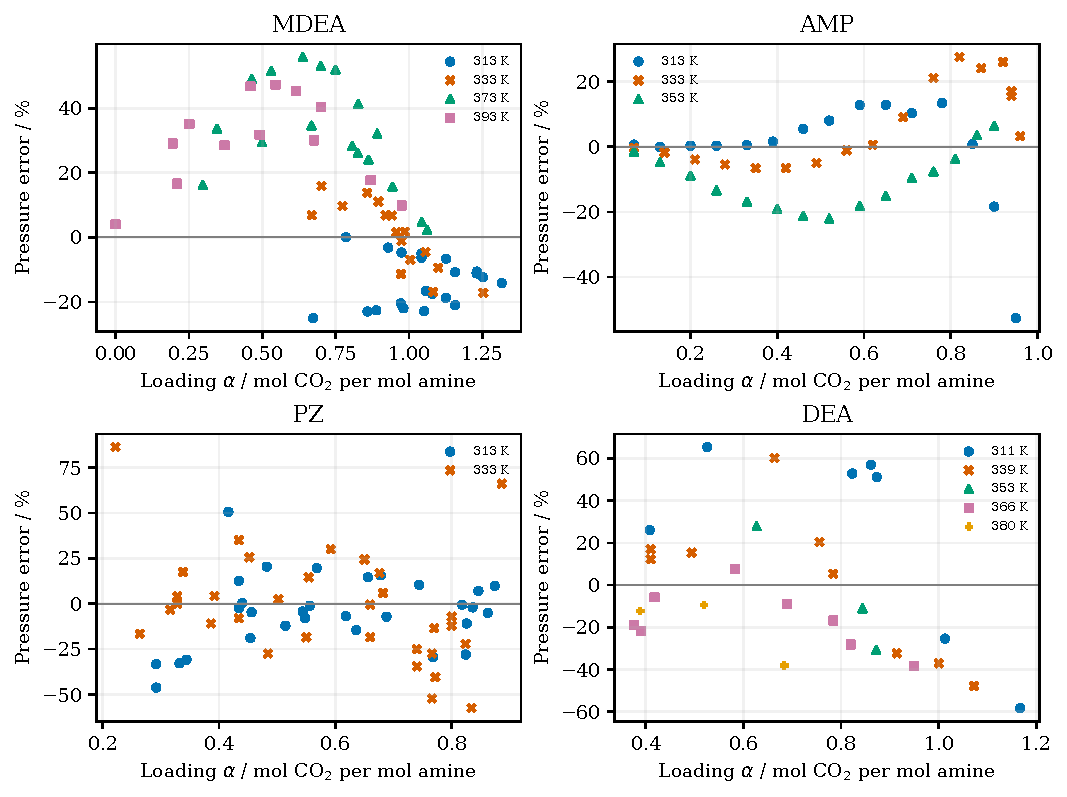
\includegraphics[width=\linewidth]{calibration.pdf}
\caption{Fitted pressure errors against analytical loading. MDEA and AMP use total pressure; PZ and DEA use \COtwo partial pressure. Each point is a calculation at a measured state. Colors distinguish source temperatures within each panel; no model curve is inferred from the discrete points. MDEA points at 373 and 393 K lie above the 368 K limit of the dissociation measurements.}
\label{fig:p2-calibration}
\end{figure}

\subsection{Unfitted pressures and reaction-law extrapolation}\label{sec:p2-unfitted}
% P:p2-results-unfitted-01
Unfitted pressure errors change with source and temperature; the largest occur in extrapolated blocks, but for MDEA, AMP and DEA they already reach 28--52\,\% AARD at conditions inside the measured law ranges.
Held-out MDEA partial-pressure AARD is 28.19\,\% over twenty Xiao observations at 23.5 wt\% and 298.15--313.15 K, all inside the dissociation law's measured range.
Every Xiao pressure is underpredicted.
The Ermatchkov aggregate, 18.27\,\% over eighty-eight observations at no more than 49 wt\%, mixes measured-law and extrapolated conditions.
Inside 278--368 K, its sixty-two pressures give 16.31\,\% AARD and $-11.59$\,\% bias; the twenty-six pressures at 393.15 K give 22.94\,\% and $+21.93$\,\%, respectively.
Fitted Kuranov total pressures exhibit the same sign reversal: 11.80\,\% AARD with $-7.80$\,\% bias inside the range, and 31.09\,\% with $+31.09$\,\% bias above it (Table~\ref{tab:p2-mdea-range}).
This is an observation about the calculated results, not a diagnosis of the dissociation law; no calculation isolates its contribution from the other temperature-dependent terms.

% Generator: docs/scientific/latex/scripts/part2_displays.py; no model evaluation.
% Input: analyses/amp_transfer/inputs/kundu/current-declarations.toml SHA256 3085081adcf6b1d5e797a49ae6b96037cc1b5bc5191f45cff699d8546d774c55
% Input: analyses/amp_transfer/inputs/redesign/refit-306-floor-coordinates.json SHA256 b8671b1abbca5c7a406147dfad2359f1c1666887fab0b4eb67e489fc80abbe99
% Input: analyses/amp_transfer/inputs/redesign/refit-306-floor-endpoint.json SHA256 6d26e1e15c89217c7e29ce1d0772aa44285158071fdf4cc1bd0f6e7fb8fb2107
% Input: analyses/amp_transfer/notebook.qmd SHA256 a46134ecc164b9304778c6d809851a64a128dd91f932e6b898da3ce04bc9fd62
% Input: analyses/amp_transfer/results/kundu/summary.json SHA256 814f2ce5a28047c470bbcab59aadf13984e7ae034b55a4239b8e5b3058d0b55e
% Input: analyses/amp_transfer/results/refit-306/kundu-pressures.csv SHA256 561d08cf41e18d6ac277ee5e2dd207904a8885274d8d45739a0ec3f56d851cdb
% Input: analyses/amp_transfer/results/refit-306/refit-306-floor-fit.json SHA256 d7ee97cb1550d2a6969de406f09048dd4326f025a79523b7e205a5c65439233c
% Input: analyses/amp_transfer/results/refit-306/summary.json SHA256 3912f54eb7821b08e05f902d3001493b269355bea383439cada4e33fc4b4128f
% Input: analyses/amp_transfer/results/refit-306/uncertainty/prediction-bands.csv SHA256 d65f885c32fc9b391305b7e0ac76ec9f0112435455d027391c66dcd1ba7a9ff0
% Input: analyses/amp_transfer/results/refit-306/uncertainty/ranking.csv SHA256 ce80d211f43c53c9f654ec85ebdd5a91ac779a827c5e992415954cacffcab2a6
% Input: analyses/dea_transfer/inputs/runs/B-2-coordinates.json SHA256 7402f93dd3334eae251b38df951d2fdc310a730bf0045871bb83482524e75beb
% Input: analyses/dea_transfer/inputs/runs/B-2-endpoint-declarations.toml SHA256 a0e6cd9a5a7796d892130fc71f756480465898fa28cb0fc8cd371e9f4b730b72
% Input: analyses/dea_transfer/inputs/runs/B-2-endpoint-document.json SHA256 91c2384ef9f7b2a035962aafb72d97435a18a94595c5f16c64c9e2ac18785cdd
% Input: analyses/dea_transfer/notebook.qmd SHA256 c08a11c9e055d810c4b04c5c421a3ac89cf9edea895c7eb2ce3225e22368373d
% Input: analyses/dea_transfer/results/figure-values.csv SHA256 58cbb7b6e6f825b0f4fba1ef19f5393ad469e8aa42a58ece391f3b3d7af4bf2c
% Input: analyses/dea_transfer/results/fits.json SHA256 b936638b0b1f83802809bea15c003c1bbcc229b23824ce61d48ac4123b80af48
% Input: analyses/dea_transfer/results/score.json SHA256 12aa281fa03ed5d34cabbe3a09174b49da105199b15f1b16087ffa33018fd64e
% Input: analyses/dea_transfer/results/uncertainty-307/prediction-bands.csv SHA256 b59d9515e2d86b3c76eea92e97343eb5b2e28512bf4e8dd9f69e359de593f9ed
% Input: analyses/dea_transfer/results/uncertainty-307/ranking.csv SHA256 14ec3184971afe521ae4be0f1d636acd3a47067df1a01feb6068d75cf63cf155
% Input: analyses/mdea_mea_workflow/notebook.qmd SHA256 55831c2a23404765f14fbcbeb2c83eb64b7245a10730ad9ad9329b85aa1c2533
% Input: analyses/mdea_mea_workflow/results/refit-298/B1-endpoint/endpoint.json SHA256 2a5341be176829d087133a1467828f762a655f92a586eb1062a5719a58142d9d
% Input: analyses/mdea_mea_workflow/results/refit-298/B1-endpoint/fitted-replay.json SHA256 6690d0b7baf4bb3f08a9437743857d965d7a4a4fd1529d4e6f8e5d234f4059e2
% Input: analyses/mdea_mea_workflow/results/refit-298/attempts.json SHA256 40e17071831a699fe380d4ac4b1b286d5d283ad434a0e704ac2803d7d22c954f
% Input: analyses/mdea_mea_workflow/results/refit-298/pressure-comparison.csv SHA256 d2cdaf4a3bc1a2b7b9b957585a6dbaec2eff15ca56c009b862dac63a2912c22c
% Input: analyses/mea_parameter_bundle/results/selected-current-best-parameters.json SHA256 f8f64820b161377a0d97d1e4ad4f6cea764cd0558dc63231d58e2096988eef97
% Input: analyses/pz_transfer/notebook.qmd SHA256 a71c49071169b4a2795c538b22d2e59c58870489e0131cecf480d5fc98622858
% Input: analyses/pz_transfer/results/holdout-A12.csv SHA256 89f6aabc166a2663ddf7be4cfdc20821cc3ef9ef46070535644f5cd2abb66b15
% Input: analyses/pz_transfer/results/reactive-A12-record.json SHA256 3eefe76e4599050e524b9a1a8354121caae0ca30de38613359cf7e1f9edc1329
% Input: analyses/pz_transfer/results/reactive-A12-residuals.csv SHA256 3c8855bba6dfaa8ed8c8e64f7c4a160cafb77fb1d85b6858e8d5520e1469e4e4
% Input: analyses/pz_transfer/results/reactive-A12-start2-endpoint.json SHA256 c24ff09badc642d5dd312f5dc03248f2e5fa4c93e3b1d91fa69fe42120297b9e
% Input: analyses/pz_transfer/results/speciation-reactions.json SHA256 64a51633b7d56ce75a1246fe51eb6a39a1f0db1abc7d75b16b2fe13df9c125be
% Input: analyses/pz_transfer/results/uncertainty-A12/ranking.csv SHA256 f266707b75ee505bb8a5226c79e6f30037696720f859ca7d239972e6f58c71fe
% Input: analyses/solvent_specification_mdea/B1-declarations.toml SHA256 7b5fd083d83731c74624707f6e9f92bad05265c9ed19d105b25cf99dd897a042
% Input: analyses/solvent_specification_mdea/inputs/B1-coordinates.json SHA256 0bca9af202313b2bd8325ccaa37a72f32a1b326099c957c5ebf35f630506c8be
% Input: analyses/solvent_specification_mdea/notebook.qmd SHA256 227db268f1475ce3e11e4873c68e3337bf217918fa0ce0bdc11deeb25f57ff88
% Input: analyses/solvent_specification_mdea/results/adoption-302/B1/pressure.json SHA256 b81bfeb21d211d64211a2bda07b5e07af2a897f828a750f01aac6142340a7820
% Input: analyses/solvent_specification_mdea/results/retained-statistics-320.json SHA256 64393229910bf06ba614d1345e1fd2d2f675e2aba1a3a9a7eaedcd33ffd07e81
% Input: analyses/solvent_specification_mdea/results/uncertainty-307/prediction-bands.csv SHA256 96fc9352b6f30dae38805b799344404528d6e49b3b45eaa42002daa8523ac0cd
% Input: analyses/solvent_specification_mdea/results/uncertainty-307/predictions.json SHA256 8fd82d94b500a2b8985ea9979e4ceb653fbfb781dc66a3d047ee68bdec0f46ba
% Input: analyses/solvent_specification_mdea/results/uncertainty-307/ranking.csv SHA256 16b4ed6165c0cc7bad4d938567c8f8e8d88bdddb3de4eb8b53c43b372f7c8e7e
% Input: docs/scientific/latex/references.bib SHA256 7dc97086df08bf802d25d2a588158a9ad3881648729bb9a5da84741ef50acd9c
% Input: docs/scientific/latex/supplement.tex SHA256 b90143f6a0711b9a7437b4845c8a5db430f8b301ff21d8f402821b105da3d5f8
\begingroup\small\setlength{\tabcolsep}{3pt}
\begin{longtable}{@{}>{\raggedright\arraybackslash}p{0.31\linewidth}>{\raggedright\arraybackslash}p{0.19\linewidth}>{\raggedright\arraybackslash}p{0.07\linewidth}>{\raggedright\arraybackslash}p{0.14\linewidth}>{\raggedright\arraybackslash}p{0.18\linewidth}@{}}
\caption{Fitted MDEA errors separated against the 278--368 K dissociation measurements. Heat signed errors are calculated minus measured; they are not relative biases.}\label{tab:p2-mdea-range}\\
\toprule Observable & Law range / $T$ & $n$ & AARD / \% & Bias / signed error \\ \midrule\endfirsthead
\toprule Observable & Law range / $T$ & $n$ & AARD / \% & Bias / signed error \\ \midrule\endhead
\bottomrule\endfoot
Kuranov total pressure & inside & $37$ & $11.80$ & $-7.80$ \\
Kuranov total pressure & outside & $30$ & $31.09$ & $31.09$ \\
Merkley heat & 333.15 K & $2$ & $10.36$ & -5725 J/mol \\
Merkley heat & 388.71 K & $2$ & $6.56$ & -3989 J/mol \\
\end{longtable}\endgroup

% Generator: docs/scientific/latex/scripts/part2_displays.py; no model evaluation.
% Input: analyses/amp_transfer/inputs/kundu/current-declarations.toml SHA256 3085081adcf6b1d5e797a49ae6b96037cc1b5bc5191f45cff699d8546d774c55
% Input: analyses/amp_transfer/inputs/redesign/refit-306-floor-coordinates.json SHA256 b8671b1abbca5c7a406147dfad2359f1c1666887fab0b4eb67e489fc80abbe99
% Input: analyses/amp_transfer/inputs/redesign/refit-306-floor-endpoint.json SHA256 6d26e1e15c89217c7e29ce1d0772aa44285158071fdf4cc1bd0f6e7fb8fb2107
% Input: analyses/amp_transfer/notebook.qmd SHA256 a46134ecc164b9304778c6d809851a64a128dd91f932e6b898da3ce04bc9fd62
% Input: analyses/amp_transfer/results/kundu/summary.json SHA256 814f2ce5a28047c470bbcab59aadf13984e7ae034b55a4239b8e5b3058d0b55e
% Input: analyses/amp_transfer/results/refit-306/kundu-pressures.csv SHA256 561d08cf41e18d6ac277ee5e2dd207904a8885274d8d45739a0ec3f56d851cdb
% Input: analyses/amp_transfer/results/refit-306/refit-306-floor-fit.json SHA256 d7ee97cb1550d2a6969de406f09048dd4326f025a79523b7e205a5c65439233c
% Input: analyses/amp_transfer/results/refit-306/summary.json SHA256 3912f54eb7821b08e05f902d3001493b269355bea383439cada4e33fc4b4128f
% Input: analyses/amp_transfer/results/refit-306/uncertainty/prediction-bands.csv SHA256 d65f885c32fc9b391305b7e0ac76ec9f0112435455d027391c66dcd1ba7a9ff0
% Input: analyses/amp_transfer/results/refit-306/uncertainty/ranking.csv SHA256 ce80d211f43c53c9f654ec85ebdd5a91ac779a827c5e992415954cacffcab2a6
% Input: analyses/dea_transfer/inputs/runs/B-2-coordinates.json SHA256 7402f93dd3334eae251b38df951d2fdc310a730bf0045871bb83482524e75beb
% Input: analyses/dea_transfer/inputs/runs/B-2-endpoint-declarations.toml SHA256 a0e6cd9a5a7796d892130fc71f756480465898fa28cb0fc8cd371e9f4b730b72
% Input: analyses/dea_transfer/inputs/runs/B-2-endpoint-document.json SHA256 91c2384ef9f7b2a035962aafb72d97435a18a94595c5f16c64c9e2ac18785cdd
% Input: analyses/dea_transfer/notebook.qmd SHA256 c08a11c9e055d810c4b04c5c421a3ac89cf9edea895c7eb2ce3225e22368373d
% Input: analyses/dea_transfer/results/figure-values.csv SHA256 58cbb7b6e6f825b0f4fba1ef19f5393ad469e8aa42a58ece391f3b3d7af4bf2c
% Input: analyses/dea_transfer/results/fits.json SHA256 b936638b0b1f83802809bea15c003c1bbcc229b23824ce61d48ac4123b80af48
% Input: analyses/dea_transfer/results/score.json SHA256 12aa281fa03ed5d34cabbe3a09174b49da105199b15f1b16087ffa33018fd64e
% Input: analyses/dea_transfer/results/uncertainty-307/prediction-bands.csv SHA256 b59d9515e2d86b3c76eea92e97343eb5b2e28512bf4e8dd9f69e359de593f9ed
% Input: analyses/dea_transfer/results/uncertainty-307/ranking.csv SHA256 14ec3184971afe521ae4be0f1d636acd3a47067df1a01feb6068d75cf63cf155
% Input: analyses/mdea_mea_workflow/notebook.qmd SHA256 55831c2a23404765f14fbcbeb2c83eb64b7245a10730ad9ad9329b85aa1c2533
% Input: analyses/mdea_mea_workflow/results/refit-298/B1-endpoint/endpoint.json SHA256 2a5341be176829d087133a1467828f762a655f92a586eb1062a5719a58142d9d
% Input: analyses/mdea_mea_workflow/results/refit-298/B1-endpoint/fitted-replay.json SHA256 6690d0b7baf4bb3f08a9437743857d965d7a4a4fd1529d4e6f8e5d234f4059e2
% Input: analyses/mdea_mea_workflow/results/refit-298/attempts.json SHA256 40e17071831a699fe380d4ac4b1b286d5d283ad434a0e704ac2803d7d22c954f
% Input: analyses/mdea_mea_workflow/results/refit-298/pressure-comparison.csv SHA256 d2cdaf4a3bc1a2b7b9b957585a6dbaec2eff15ca56c009b862dac63a2912c22c
% Input: analyses/mea_parameter_bundle/results/selected-current-best-parameters.json SHA256 f8f64820b161377a0d97d1e4ad4f6cea764cd0558dc63231d58e2096988eef97
% Input: analyses/pz_transfer/notebook.qmd SHA256 0b5d7fe8f2e9f417972f8998257cb5108325815a49eecda383e59ef740770bae
% Input: analyses/pz_transfer/results/check-states-A12-direct.json SHA256 b5d7c54a1c14c62b090776b12c8cb8c28bbfa658fa7e87d735dd778078f5d056
% Input: analyses/pz_transfer/results/check-states-A12.json SHA256 61664db83e7284fdc2aaa6961fd3fd23c99864e6fe79b192d93e2b07f25e2530
% Input: analyses/pz_transfer/results/holdout-A12.csv SHA256 89f6aabc166a2663ddf7be4cfdc20821cc3ef9ef46070535644f5cd2abb66b15
% Input: analyses/pz_transfer/results/kamps2003-A12.csv SHA256 34f8300ca39e4a25c77f1bc834d2c22198f0ace06a4dda28ecc82eacba7bfe84
% Input: analyses/pz_transfer/results/kamps2003-A12.json SHA256 bb5f044833c67ad7b9bf911c14cf5d9b7a0d6f0c894ba8a697062250708439b9
% Input: analyses/pz_transfer/results/reactive-A12-record.json SHA256 3eefe76e4599050e524b9a1a8354121caae0ca30de38613359cf7e1f9edc1329
% Input: analyses/pz_transfer/results/reactive-A12-residuals.csv SHA256 3c8855bba6dfaa8ed8c8e64f7c4a160cafb77fb1d85b6858e8d5520e1469e4e4
% Input: analyses/pz_transfer/results/reactive-A12-start2-endpoint.json SHA256 c24ff09badc642d5dd312f5dc03248f2e5fa4c93e3b1d91fa69fe42120297b9e
% Input: analyses/pz_transfer/results/speciation-reactions.json SHA256 64a51633b7d56ce75a1246fe51eb6a39a1f0db1abc7d75b16b2fe13df9c125be
% Input: analyses/pz_transfer/results/uncertainty-A12/ranking.csv SHA256 f266707b75ee505bb8a5226c79e6f30037696720f859ca7d239972e6f58c71fe
% Input: analyses/solvent_specification_mdea/B1-declarations.toml SHA256 7b5fd083d83731c74624707f6e9f92bad05265c9ed19d105b25cf99dd897a042
% Input: analyses/solvent_specification_mdea/inputs/B1-coordinates.json SHA256 0bca9af202313b2bd8325ccaa37a72f32a1b326099c957c5ebf35f630506c8be
% Input: analyses/solvent_specification_mdea/notebook.qmd SHA256 227db268f1475ce3e11e4873c68e3337bf217918fa0ce0bdc11deeb25f57ff88
% Input: analyses/solvent_specification_mdea/results/adoption-302/B1/pressure.json SHA256 b81bfeb21d211d64211a2bda07b5e07af2a897f828a750f01aac6142340a7820
% Input: analyses/solvent_specification_mdea/results/retained-statistics-320.json SHA256 64393229910bf06ba614d1345e1fd2d2f675e2aba1a3a9a7eaedcd33ffd07e81
% Input: analyses/solvent_specification_mdea/results/uncertainty-307/prediction-bands.csv SHA256 96fc9352b6f30dae38805b799344404528d6e49b3b45eaa42002daa8523ac0cd
% Input: analyses/solvent_specification_mdea/results/uncertainty-307/predictions.json SHA256 8fd82d94b500a2b8985ea9979e4ceb653fbfb781dc66a3d047ee68bdec0f46ba
% Input: analyses/solvent_specification_mdea/results/uncertainty-307/ranking.csv SHA256 16b4ed6165c0cc7bad4d938567c8f8e8d88bdddb3de4eb8b53c43b372f7c8e7e
% Input: docs/scientific/latex/references.bib SHA256 dc2b40df7e47ccd8bc493e8d407c79d79bc8a302924bbd2d5f8cdf4320759e17
% Input: docs/scientific/latex/supplement.tex SHA256 b90143f6a0711b9a7437b4845c8a5db430f8b301ff21d8f402821b105da3d5f8
\begingroup\small\setlength{\tabcolsep}{3pt}
\begin{longtable}{@{}>{\raggedright\arraybackslash}p{0.2\linewidth}>{\raggedright\arraybackslash}p{0.15\linewidth}>{\raggedright\arraybackslash}p{0.04\linewidth}>{\raggedright\arraybackslash}p{0.1\linewidth}>{\raggedright\arraybackslash}p{0.1\linewidth}>{\raggedright\arraybackslash}p{0.29\linewidth}@{}}
\caption{Unfitted pressure errors by source and temperature. MDEA sets were previously accessed; AMP Kundu and PZ Ermatchkov were scored before final parameter selection, and DEA was first scored on a numerically tied fit. Kamps was scored once after the PZ fit was frozen. All are partial pressures except AMP Tong and PZ Kamps.}\label{tab:p2-unfitted}\\
\toprule Amine and source & Conditions & $n$ & AARD / \% & Bias / \% & Measured-law range \\ \midrule\endfirsthead
\toprule Amine and source & Conditions & $n$ & AARD / \% & Bias / \% & Measured-law range \\ \midrule\endhead
\bottomrule\endfoot
MDEA Xiao & all & $20$ & $28.19$ & $-28.19$ & inside \\
MDEA Ermatchkov & all & $88$ & $18.27$ & $-1.68$ & mixed \\
MDEA Ermatchkov & 278--368 K & $62$ & $16.31$ & $-11.59$ & inside \\
MDEA Ermatchkov & above 368 K & $26$ & $22.94$ & $21.93$ & dissociation extrapolated \\
AMP Kundu & all & $51$ & $42.85$ & $37.79$ & mixed \\
AMP Kundu & 303.0 K & $25$ & $53.94$ & $53.94$ & hydrolysis slope extrapolated \\
AMP Kundu & 313.0 K & $15$ & $43.78$ & $43.78$ & inside \\
AMP Kundu & 323.0 K & $11$ & $16.35$ & $-7.09$ & inside \\
AMP Tong (total) & 313--353 K & $17$ & $28.66$ & $8.11$ & inside \\
PZ Ermatchkov & all & $52$ & $21.94$ & $7.82$ & mixed \\
PZ Ermatchkov & 313.1 K & $19$ & $9.32$ & $-8.70$ & inside \\
PZ Ermatchkov & 353.15 K & $18$ & $13.12$ & $-8.64$ & carbamate extrapolated \\
PZ Ermatchkov & 393.15 K & $15$ & $48.52$ & $48.52$ & carbamate and protonation extrapolated \\
DEA Seo \& Hong & all & $16$ & $79.54$ & $77.80$ & mixed \\
DEA Seo \& Hong & 40$\,^{\circ}$C & $5$ & $28.51$ & $22.95$ & inside \\
DEA Seo \& Hong & 60$\,^{\circ}$C & $6$ & $59.82$ & $59.82$ & protonation extrapolated \\
DEA Seo \& Hong & 80$\,^{\circ}$C & $5$ & $154.22$ & $154.22$ & protonation extrapolated \\
DEA Lal & all & $44$ & $44.17$ & $-22.93$ & mixed \\
DEA Lal & 40$\,^{\circ}$C & $17$ & $52.25$ & $-48.61$ & inside \\
DEA Lal & 100$\,^{\circ}$C & $27$ & $39.09$ & $-6.76$ & protonation extrapolated \\
PZ Kamps (total) & all & $94$ & $42.5$ & $-40.3$ & mixed; comparison-only \\
\end{longtable}\endgroup


% P:p2-results-unfitted-02
The reported AMP fit gives Kundu AARD 42.85\,\% and bias $+37.79$\,\% over all fifty-one observations.
The signed error decreases with temperature: $+53.94$\,\% at 303 K, $+43.78$\,\% at 313 K and $-7.09$\,\% at 323 K.
The 303 K set extrapolates the source basis of the hydrolysis slope below 313 K; all three temperatures are within the fixed dissociation law's interval.
Tong's seventeen total pressures \cite{Tong2012} at 313--353 K give 28.66\,\% AARD and $+8.11$\,\% bias, while twenty-three rows at 373--393 K lie above the dissociation law's declared 353.22 K limit and are not calculated.
The Tong biases also decrease with temperature, from $+48.55$ through $+5.73$ to $-23.19$\,\% at approximately 313, 333 and 353 K.
The decreasing signed errors and bound hydrolysis enthalpy correction are relevant to temperature dependence, but do not distinguish model error from disagreement between experiments.

% P:p2-results-unfitted-03
PZ Ermatchkov partial pressures \cite{ermatchkovSolubilityCarbonDioxide2006a} give 21.94\,\% AARD overall, with strong temperature dependence.
At 313.1 K, within the carbamate measurements, AARD is 9.32\,\%; at 353.15 K, above those measurements, it is 13.12\,\%; at 393.15 K, above both carbamate and protonation measurements, it reaches 48.52\,\%.

Only eleven of fifty-two pressures lie within the printed source uncertainty, and the uncertainty-scaled RMS is 11.59.
The mean error consequently understates the disagreement relative to the source's measurement resolution.

% P:p2-results-kamps-01
The comparison-only total pressures of P\'erez-Salado Kamps et al. \cite[Table~3, p.~2666]{kampsSolubilityCO2H2O+piperazine2003a} were scored once on the frozen twelve-coordinate PZ fit and never fitted or used to select it.
The ninety-four rows give 42.5\,\% AARD and $-40.3$\,\% bias.
Loaded rows below 0.2 MPa give 20.4\,\% AARD and $-6.0$\,\% bias; the loaded 374--395 K rows at or above 0.2 MPa give 37.1\,\% and $-35.2$\,\%, and the remaining loaded 313--354 K rows give 53.0\,\% and $-53.0$\,\%.
The 313.75 K block, inside both the 283.15--333.15 K carbamate and 293.14--353.42 K protonation measurements, still has $-32.1$\,\% bias, so leaving those ranges is not the only cause.
Only that block lies inside both PZ laws; the 395.0 K rows also exceed the shared R2 interval (Supplementary Table~\ref{supp-tab:p2-kamps-blocks}).

% P:p2-results-kamps-02
The source gives pressure bounds of $\pm4$ or $\pm10$ kPa, without assigning the transducer to each row, and uncertainty up to 10\,\% below 0.1 MPa \cite[pp.~2664, 2667]{kampsSolubilityCO2H2O+piperazine2003a}.
All eighty-two loaded rows at or above 0.2 MPa lie outside both pressure bounds.
The $\pm0.7$\,\% solvent-mass bound moves calculated pressure by up to $-10.8$\,\% / $+11.7$\,\%; the median ratio of sensitivity to misfit is 0.07 and the maximum is 0.88.
Near 1 mol/mol at low pressure this sensitivity can be comparable to the misfit, but for thirty rows above 1.2 mol/mol and at or above 0.2 MPa it is at most 3.2\,\% against misfits of at least 34.9\,\%.
These are input sensitivities, not propagated total uncertainties; the individual charged \COtwo masses needed to propagate their uncertainty were not reported.

% P:p2-results-unfitted-04
DEA predicts Seo and Hong's thirty-mass-percent solution \cite{seoSolubilitiesCarbonDioxide1996} with 79.54\,\% AARD and $+77.80$\,\% bias; the 80 $^{\circ}$C subset reaches 154.22\,\%.
Lal's more dilute stock \cite{lalSolubilityH2SCO21985} instead gives 44.17\,\% AARD and $-22.93$\,\% bias.
Even the 40 $^{\circ}$C subsets, within the Bower measured temperature range, have AARDs 28.51\,\% against Seo and Hong and 52.25\,\% against Lal.
The higher-temperature subsets extrapolate that law, with the source-specific errors listed in Table~\ref{tab:p2-unfitted}.
Lal's low-pressure observations, which the source reports as less accurate, remain in the AARD (Supplementary Section~S4).

% P:p2-results-unfitted-05
The source tables indicate a possible contribution from laboratory disagreement in DEA.
At loading about 0.41, Lawson reports 16.0--16.7 kPa at 65.6 $^{\circ}$C and 25 wt\%, while Seo and Hong report 11.6 kPa at 80 $^{\circ}$C and 30 wt\%.
These are not matched states: temperature, concentration and loading differ.
They do not isolate experimental bias or establish which source is correct, and the model retains a loading-shape error within its own fitted source.
Across amines, unmatched pressure types, source uncertainties, concentrations, temperatures and selection histories prevent comparison of their error percentages as an accuracy ranking.

\begin{figure}[pos=!htbp]
\centering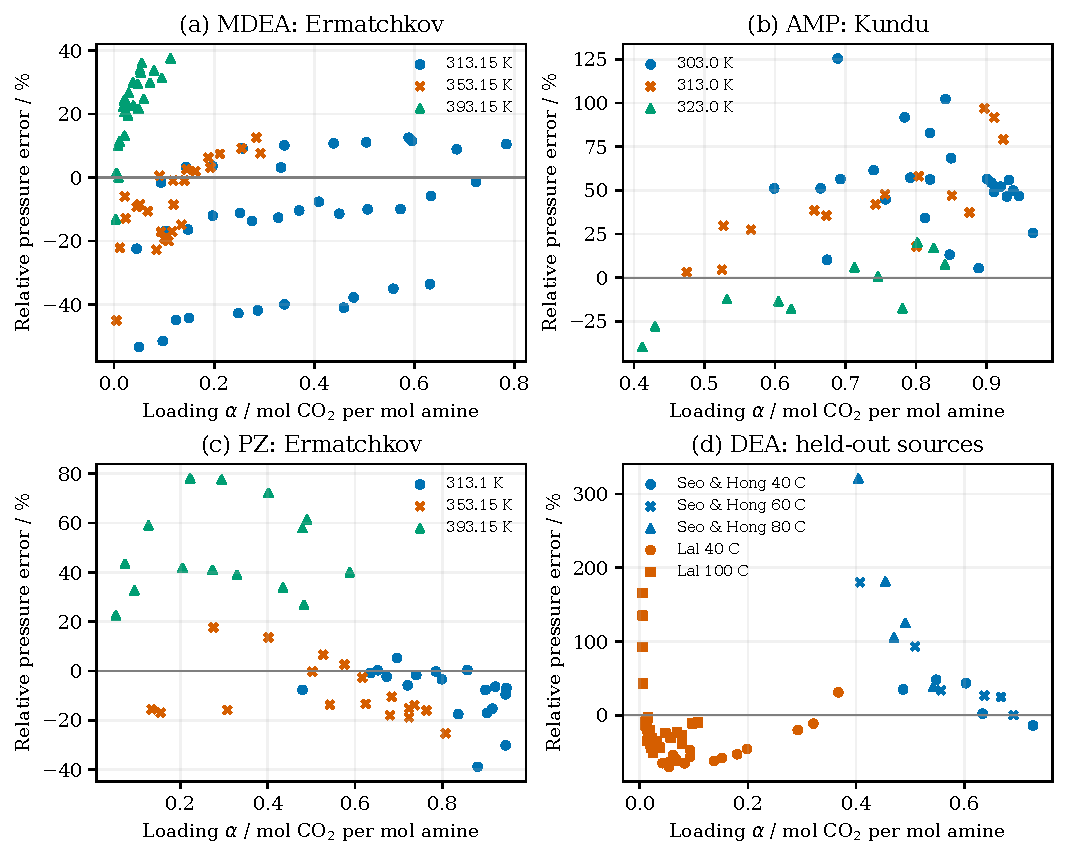
\includegraphics[width=\linewidth]{unfitted-pressure.pdf}
\caption{Relative partial-pressure errors at measured loadings. All panels use held-out sets; the MDEA set was previously accessed. MDEA at 393.15 K exceeds its dissociation measurements; PZ at 353.15 K exceeds its carbamate measurements and at 393.15 K also its protonation measurements; AMP at 303 K extrapolates the hydrolysis source slope. DEA marker shapes distinguish 40, 60, 80 and 100 $^{\circ}$C. Points from different stocks are shown without interpolating a continuous relation.}
\label{fig:p2-unfitted}
\end{figure}
\FloatBarrier

\subsection{Conditional parameter uncertainty beside the unfitted errors}\label{sec:p2-uncertainty}
% P:p2-results-uncertainty-01
For AMP and DEA, conditional parameter bands are far smaller than the observed unfitted-pressure errors (Fig.~\ref{fig:p2-bands}).
AMP Kundu relative SEs range from 3.2 to 13.5\,\%, with median 6.7\,\%; only eight of fifty-one observations fall within the nominal $\pm1.96$ SE intervals.
DEA relative pressure SEs are 5.4--11.6\,\% for Seo and Hong and 12.3--19.1\,\% for Lal, compared with their much larger measured deviations.
These comparisons show that uncertainty within the selected local parameter fit does not encompass the discrepancies.
They do not identify which experiment or model term causes a miss.

% P:p2-results-uncertainty-02
MDEA bands at the 108 Xiao and Ermatchkov pressure states have relative SEs of 7.82--39.1\,\%, overlapping the magnitude of the held-out errors.
Its cation--bicarbonate interaction and cation Born diameter lie at $+1$ and 7 \AA, respectively, and remain fixed in this covariance.
For AMP, the carbamate diameter and hydrolysis enthalpy correction are fixed at their limits, 5.32 \AA\ and $-5000$ J/mol.
The corresponding residual-variance factors are 2.7639784 for MDEA and 0.829 for AMP.
The band size therefore depends on both the fitted information and the conditional error model, not just the parameter count.

% P:p2-results-uncertainty-03
PZ's local linear uncertainty is less reliable: one marginal SE of a fitted dispersion energy changes some Hilliard calibration pressures by 90--160\,\% in the linear estimate.
Its cation--bicarbonate interaction is $-0.02\pm1.03$ across an allowed interval of width 1.5, indicating weak identification.
With the PZH$^+$--water interaction fixed at its $-1$ limit, eleven interior coordinates use variance factor 146.3; calibration-pressure relative SEs range from 2.8 to 34\,\%.
No PZ held-out pressure band was calculated, and the calibration band cannot substitute for it.
The inward 5 and 10\,\% profile refits did not converge, so their costs are upper bounds.

% P:p2-results-uncertainty-04
DEA has no active parameter bounds, but its hydrolysis-law level and carbamate--water interaction have correlation 0.972.
Its residual-variance factor is 0.210, and relative SEs at fitted Lawson and Carson states are 3.3--10.3\,\% and 0.9--1.9\,\%, respectively.
Small conditional errors coexist with compensation between parameters.
Supplementary Section~S6 reports all parameter SEs, sensitivity definitions and inward profiles.
None includes shared-input uncertainty, experimental systematic errors, uncertainty in the omitted chemistry or model discrepancy.

\begin{figure}[pos=!htbp]
\centering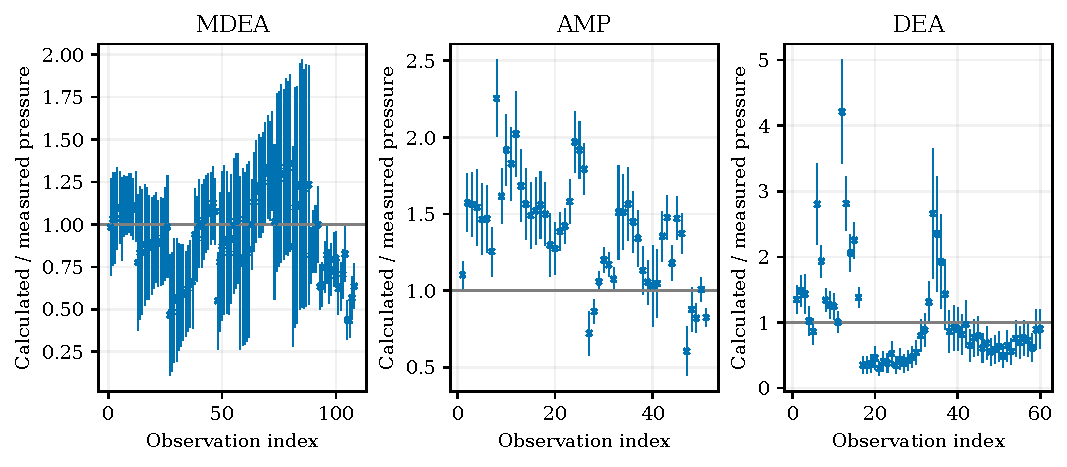
\includegraphics[width=\linewidth]{pressure-bands.pdf}
\caption{Calculated-to-measured partial-pressure ratios with nominal $\pm1.96$ conditional parameter-SE intervals, at stored measured states. Separate panels show MDEA Xiao/Ermatchkov, AMP Kundu and DEA Seo and Hong/Lal; the horizontal axis numbers the observations within each panel and is not a temperature or loading axis. The horizontal line is equality. Intervals are linear parameter propagation, conditional on fixed shared inputs and active bounds; they exclude measurement noise and model discrepancy. PZ held-out bands are unavailable.}
\label{fig:p2-bands}
\end{figure}

\subsection{Sensitivity of unfitted pressures to the shared description}\label{sec:p2-shared-sensitivity}
% P:p2-results-sensitivity-01
Unfitted pressures depend on the shared description as well as on the amine fit: substituting Part I's bicarbonate--water interaction and R2 law moves the MDEA and AMP errors by 22--26 percentage points in opposite directions before the amine parameters are refitted (Table~\ref{tab:p2-shared-sensitivity}).
Table~\ref{tab:p2-shared-sensitivity} follows the same data through the earlier shared description, substitution of the Part I bicarbonate--water interaction and fitted R2 law, and amine-specific refitting.
For AMP, Kundu AARD changes from 43.69 to 21.89\,\% upon substitution without refitting, then returns to 43.51\,\% when the original AMP coordinates and limits are refitted.
The substitution worsens fitted total-pressure AARD to 18.85\,\%, while refitting recovers 9.93\,\%.
The favorable 21.89\,\% score thus reflects cancelling changes in this comparison, not a jointly improved calibration and independent pressure description.

% Generator: docs/scientific/latex/scripts/part2_displays.py; no model evaluation.
% Input: analyses/amp_transfer/inputs/kundu/current-declarations.toml SHA256 3085081adcf6b1d5e797a49ae6b96037cc1b5bc5191f45cff699d8546d774c55
% Input: analyses/amp_transfer/inputs/redesign/refit-306-floor-coordinates.json SHA256 b8671b1abbca5c7a406147dfad2359f1c1666887fab0b4eb67e489fc80abbe99
% Input: analyses/amp_transfer/inputs/redesign/refit-306-floor-endpoint.json SHA256 6d26e1e15c89217c7e29ce1d0772aa44285158071fdf4cc1bd0f6e7fb8fb2107
% Input: analyses/amp_transfer/notebook.qmd SHA256 a46134ecc164b9304778c6d809851a64a128dd91f932e6b898da3ce04bc9fd62
% Input: analyses/amp_transfer/results/kundu/summary.json SHA256 814f2ce5a28047c470bbcab59aadf13984e7ae034b55a4239b8e5b3058d0b55e
% Input: analyses/amp_transfer/results/refit-306/kundu-pressures.csv SHA256 561d08cf41e18d6ac277ee5e2dd207904a8885274d8d45739a0ec3f56d851cdb
% Input: analyses/amp_transfer/results/refit-306/refit-306-floor-fit.json SHA256 d7ee97cb1550d2a6969de406f09048dd4326f025a79523b7e205a5c65439233c
% Input: analyses/amp_transfer/results/refit-306/summary.json SHA256 3912f54eb7821b08e05f902d3001493b269355bea383439cada4e33fc4b4128f
% Input: analyses/amp_transfer/results/refit-306/uncertainty/prediction-bands.csv SHA256 d65f885c32fc9b391305b7e0ac76ec9f0112435455d027391c66dcd1ba7a9ff0
% Input: analyses/amp_transfer/results/refit-306/uncertainty/ranking.csv SHA256 ce80d211f43c53c9f654ec85ebdd5a91ac779a827c5e992415954cacffcab2a6
% Input: analyses/dea_transfer/inputs/runs/B-2-coordinates.json SHA256 7402f93dd3334eae251b38df951d2fdc310a730bf0045871bb83482524e75beb
% Input: analyses/dea_transfer/inputs/runs/B-2-endpoint-declarations.toml SHA256 a0e6cd9a5a7796d892130fc71f756480465898fa28cb0fc8cd371e9f4b730b72
% Input: analyses/dea_transfer/inputs/runs/B-2-endpoint-document.json SHA256 91c2384ef9f7b2a035962aafb72d97435a18a94595c5f16c64c9e2ac18785cdd
% Input: analyses/dea_transfer/notebook.qmd SHA256 c08a11c9e055d810c4b04c5c421a3ac89cf9edea895c7eb2ce3225e22368373d
% Input: analyses/dea_transfer/results/figure-values.csv SHA256 58cbb7b6e6f825b0f4fba1ef19f5393ad469e8aa42a58ece391f3b3d7af4bf2c
% Input: analyses/dea_transfer/results/fits.json SHA256 b936638b0b1f83802809bea15c003c1bbcc229b23824ce61d48ac4123b80af48
% Input: analyses/dea_transfer/results/score.json SHA256 12aa281fa03ed5d34cabbe3a09174b49da105199b15f1b16087ffa33018fd64e
% Input: analyses/dea_transfer/results/uncertainty-307/prediction-bands.csv SHA256 b59d9515e2d86b3c76eea92e97343eb5b2e28512bf4e8dd9f69e359de593f9ed
% Input: analyses/dea_transfer/results/uncertainty-307/ranking.csv SHA256 14ec3184971afe521ae4be0f1d636acd3a47067df1a01feb6068d75cf63cf155
% Input: analyses/mdea_mea_workflow/notebook.qmd SHA256 55831c2a23404765f14fbcbeb2c83eb64b7245a10730ad9ad9329b85aa1c2533
% Input: analyses/mdea_mea_workflow/results/refit-298/B1-endpoint/endpoint.json SHA256 2a5341be176829d087133a1467828f762a655f92a586eb1062a5719a58142d9d
% Input: analyses/mdea_mea_workflow/results/refit-298/B1-endpoint/fitted-replay.json SHA256 6690d0b7baf4bb3f08a9437743857d965d7a4a4fd1529d4e6f8e5d234f4059e2
% Input: analyses/mdea_mea_workflow/results/refit-298/attempts.json SHA256 40e17071831a699fe380d4ac4b1b286d5d283ad434a0e704ac2803d7d22c954f
% Input: analyses/mdea_mea_workflow/results/refit-298/pressure-comparison.csv SHA256 d2cdaf4a3bc1a2b7b9b957585a6dbaec2eff15ca56c009b862dac63a2912c22c
% Input: analyses/mea_parameter_bundle/results/selected-current-best-parameters.json SHA256 f8f64820b161377a0d97d1e4ad4f6cea764cd0558dc63231d58e2096988eef97
% Input: analyses/pz_transfer/notebook.qmd SHA256 0b5d7fe8f2e9f417972f8998257cb5108325815a49eecda383e59ef740770bae
% Input: analyses/pz_transfer/results/check-states-A12-direct.json SHA256 b5d7c54a1c14c62b090776b12c8cb8c28bbfa658fa7e87d735dd778078f5d056
% Input: analyses/pz_transfer/results/check-states-A12.json SHA256 61664db83e7284fdc2aaa6961fd3fd23c99864e6fe79b192d93e2b07f25e2530
% Input: analyses/pz_transfer/results/holdout-A12.csv SHA256 89f6aabc166a2663ddf7be4cfdc20821cc3ef9ef46070535644f5cd2abb66b15
% Input: analyses/pz_transfer/results/kamps2003-A12.csv SHA256 34f8300ca39e4a25c77f1bc834d2c22198f0ace06a4dda28ecc82eacba7bfe84
% Input: analyses/pz_transfer/results/kamps2003-A12.json SHA256 bb5f044833c67ad7b9bf911c14cf5d9b7a0d6f0c894ba8a697062250708439b9
% Input: analyses/pz_transfer/results/reactive-A12-record.json SHA256 3eefe76e4599050e524b9a1a8354121caae0ca30de38613359cf7e1f9edc1329
% Input: analyses/pz_transfer/results/reactive-A12-residuals.csv SHA256 3c8855bba6dfaa8ed8c8e64f7c4a160cafb77fb1d85b6858e8d5520e1469e4e4
% Input: analyses/pz_transfer/results/reactive-A12-start2-endpoint.json SHA256 c24ff09badc642d5dd312f5dc03248f2e5fa4c93e3b1d91fa69fe42120297b9e
% Input: analyses/pz_transfer/results/speciation-reactions.json SHA256 64a51633b7d56ce75a1246fe51eb6a39a1f0db1abc7d75b16b2fe13df9c125be
% Input: analyses/pz_transfer/results/uncertainty-A12/ranking.csv SHA256 f266707b75ee505bb8a5226c79e6f30037696720f859ca7d239972e6f58c71fe
% Input: analyses/solvent_specification_mdea/B1-declarations.toml SHA256 7b5fd083d83731c74624707f6e9f92bad05265c9ed19d105b25cf99dd897a042
% Input: analyses/solvent_specification_mdea/inputs/B1-coordinates.json SHA256 0bca9af202313b2bd8325ccaa37a72f32a1b326099c957c5ebf35f630506c8be
% Input: analyses/solvent_specification_mdea/notebook.qmd SHA256 227db268f1475ce3e11e4873c68e3337bf217918fa0ce0bdc11deeb25f57ff88
% Input: analyses/solvent_specification_mdea/results/adoption-302/B1/pressure.json SHA256 b81bfeb21d211d64211a2bda07b5e07af2a897f828a750f01aac6142340a7820
% Input: analyses/solvent_specification_mdea/results/retained-statistics-320.json SHA256 64393229910bf06ba614d1345e1fd2d2f675e2aba1a3a9a7eaedcd33ffd07e81
% Input: analyses/solvent_specification_mdea/results/uncertainty-307/prediction-bands.csv SHA256 96fc9352b6f30dae38805b799344404528d6e49b3b45eaa42002daa8523ac0cd
% Input: analyses/solvent_specification_mdea/results/uncertainty-307/predictions.json SHA256 8fd82d94b500a2b8985ea9979e4ceb653fbfb781dc66a3d047ee68bdec0f46ba
% Input: analyses/solvent_specification_mdea/results/uncertainty-307/ranking.csv SHA256 16b4ed6165c0cc7bad4d938567c8f8e8d88bdddb3de4eb8b53c43b372f7c8e7e
% Input: docs/scientific/latex/references.bib SHA256 9ac4ac1c25d01550aa5e9a9df066b7a49e96212687fb4c6f9c826ee81cea4252
% Input: docs/scientific/latex/supplement.tex SHA256 b90143f6a0711b9a7437b4845c8a5db430f8b301ff21d8f402821b105da3d5f8
\begingroup\small\setlength{\tabcolsep}{3pt}
\begin{longtable}{@{}>{\raggedright\arraybackslash}p{0.48\linewidth}>{\raggedright\arraybackslash}p{0.13\linewidth}>{\raggedright\arraybackslash}p{0.13\linewidth}>{\raggedright\arraybackslash}p{0.13\linewidth}@{}}
\caption{Same-data pressure AARD (\%). Each row compares the earlier shared inputs, substitution of the Part I bicarbonate--water interaction and R2 law without refitting the amine, then amine-specific refitting. A3 is a counter-case, not the selected MDEA description. AMP here uses the original bounds; its final bounded fit is reported separately.}\label{tab:p2-shared-sensitivity}\\
\toprule Amine fit (unfitted source) & Earlier & Substituted & Refitted \\ \midrule\endfirsthead
\toprule Amine fit (unfitted source) & Earlier & Substituted & Refitted \\ \midrule\endhead
\bottomrule\endfoot
MDEA alternative ion description A3 (Ermatchkov) & $26.21$ & $52.47$ & $31.44$ \\
MDEA reported fit (Ermatchkov) & $19.15$ & $42.03$ & $18.27$ \\
AMP (Kundu) & $43.69$ & $21.89$ & $43.51$ \\
\end{longtable}\endgroup


% P:p2-results-sensitivity-02
For the reported MDEA fit, the same sequence changes Ermatchkov AARD from 19.15 to 42.03 and then 18.27\,\%.
An alternative MDEA ion description, A3, changes from 26.21 to 52.47 and then 31.44\,\%, so refitting does not recover its earlier error.
A3 is a counter-case, not an additional selected model.
These same-source interventions demonstrate parameter compensation but do not uniquely assign the discrepancy to bicarbonate, Born solvation or a reaction constant.

% P:p2-results-sensitivity-03
The reported AMP fit widens the cation--\COtwo interaction and retains the 5.32 \AA\ carbamate floor, giving 42.85\,\% Kundu AARD.
Lowering the floor to 3.5 \AA\ gives a slightly smaller calibration cost but 43.95\,\% Kundu AARD; it is not the reported result.
Supplementary Section~S7 gives the complete sequence.
A model-free comparison of the Hartono and Kundu measurements lacks sufficient matched conditions, especially at 303 K, to decide whether Hartono and Kundu disagree or whether the model misses their concentration dependence.
Its interpolation and vapor-baseline assumptions do not establish that either source is erroneous.
\FloatBarrier

\subsection{Comparison with published models}\label{sec:p2-literature}
% Generator: docs/scientific/latex/scripts/part2_displays.py; no model evaluation.
% Input: analyses/amp_transfer/inputs/kundu/current-declarations.toml SHA256 3085081adcf6b1d5e797a49ae6b96037cc1b5bc5191f45cff699d8546d774c55
% Input: analyses/amp_transfer/inputs/redesign/refit-306-floor-coordinates.json SHA256 b8671b1abbca5c7a406147dfad2359f1c1666887fab0b4eb67e489fc80abbe99
% Input: analyses/amp_transfer/inputs/redesign/refit-306-floor-endpoint.json SHA256 6d26e1e15c89217c7e29ce1d0772aa44285158071fdf4cc1bd0f6e7fb8fb2107
% Input: analyses/amp_transfer/notebook.qmd SHA256 a46134ecc164b9304778c6d809851a64a128dd91f932e6b898da3ce04bc9fd62
% Input: analyses/amp_transfer/results/kundu/summary.json SHA256 814f2ce5a28047c470bbcab59aadf13984e7ae034b55a4239b8e5b3058d0b55e
% Input: analyses/amp_transfer/results/refit-306/kundu-pressures.csv SHA256 561d08cf41e18d6ac277ee5e2dd207904a8885274d8d45739a0ec3f56d851cdb
% Input: analyses/amp_transfer/results/refit-306/refit-306-floor-fit.json SHA256 d7ee97cb1550d2a6969de406f09048dd4326f025a79523b7e205a5c65439233c
% Input: analyses/amp_transfer/results/refit-306/summary.json SHA256 3912f54eb7821b08e05f902d3001493b269355bea383439cada4e33fc4b4128f
% Input: analyses/amp_transfer/results/refit-306/uncertainty/prediction-bands.csv SHA256 d65f885c32fc9b391305b7e0ac76ec9f0112435455d027391c66dcd1ba7a9ff0
% Input: analyses/amp_transfer/results/refit-306/uncertainty/ranking.csv SHA256 ce80d211f43c53c9f654ec85ebdd5a91ac779a827c5e992415954cacffcab2a6
% Input: analyses/dea_transfer/inputs/runs/B-2-coordinates.json SHA256 7402f93dd3334eae251b38df951d2fdc310a730bf0045871bb83482524e75beb
% Input: analyses/dea_transfer/inputs/runs/B-2-endpoint-declarations.toml SHA256 a0e6cd9a5a7796d892130fc71f756480465898fa28cb0fc8cd371e9f4b730b72
% Input: analyses/dea_transfer/inputs/runs/B-2-endpoint-document.json SHA256 91c2384ef9f7b2a035962aafb72d97435a18a94595c5f16c64c9e2ac18785cdd
% Input: analyses/dea_transfer/notebook.qmd SHA256 c08a11c9e055d810c4b04c5c421a3ac89cf9edea895c7eb2ce3225e22368373d
% Input: analyses/dea_transfer/results/figure-values.csv SHA256 58cbb7b6e6f825b0f4fba1ef19f5393ad469e8aa42a58ece391f3b3d7af4bf2c
% Input: analyses/dea_transfer/results/fits.json SHA256 b936638b0b1f83802809bea15c003c1bbcc229b23824ce61d48ac4123b80af48
% Input: analyses/dea_transfer/results/score.json SHA256 12aa281fa03ed5d34cabbe3a09174b49da105199b15f1b16087ffa33018fd64e
% Input: analyses/dea_transfer/results/uncertainty-307/prediction-bands.csv SHA256 b59d9515e2d86b3c76eea92e97343eb5b2e28512bf4e8dd9f69e359de593f9ed
% Input: analyses/dea_transfer/results/uncertainty-307/ranking.csv SHA256 14ec3184971afe521ae4be0f1d636acd3a47067df1a01feb6068d75cf63cf155
% Input: analyses/mdea_mea_workflow/notebook.qmd SHA256 55831c2a23404765f14fbcbeb2c83eb64b7245a10730ad9ad9329b85aa1c2533
% Input: analyses/mdea_mea_workflow/results/refit-298/B1-endpoint/endpoint.json SHA256 2a5341be176829d087133a1467828f762a655f92a586eb1062a5719a58142d9d
% Input: analyses/mdea_mea_workflow/results/refit-298/B1-endpoint/fitted-replay.json SHA256 6690d0b7baf4bb3f08a9437743857d965d7a4a4fd1529d4e6f8e5d234f4059e2
% Input: analyses/mdea_mea_workflow/results/refit-298/attempts.json SHA256 40e17071831a699fe380d4ac4b1b286d5d283ad434a0e704ac2803d7d22c954f
% Input: analyses/mdea_mea_workflow/results/refit-298/pressure-comparison.csv SHA256 d2cdaf4a3bc1a2b7b9b957585a6dbaec2eff15ca56c009b862dac63a2912c22c
% Input: analyses/mea_parameter_bundle/results/selected-current-best-parameters.json SHA256 f8f64820b161377a0d97d1e4ad4f6cea764cd0558dc63231d58e2096988eef97
% Input: analyses/pz_transfer/notebook.qmd SHA256 a71c49071169b4a2795c538b22d2e59c58870489e0131cecf480d5fc98622858
% Input: analyses/pz_transfer/results/holdout-A12.csv SHA256 89f6aabc166a2663ddf7be4cfdc20821cc3ef9ef46070535644f5cd2abb66b15
% Input: analyses/pz_transfer/results/reactive-A12-record.json SHA256 3eefe76e4599050e524b9a1a8354121caae0ca30de38613359cf7e1f9edc1329
% Input: analyses/pz_transfer/results/reactive-A12-residuals.csv SHA256 3c8855bba6dfaa8ed8c8e64f7c4a160cafb77fb1d85b6858e8d5520e1469e4e4
% Input: analyses/pz_transfer/results/reactive-A12-start2-endpoint.json SHA256 c24ff09badc642d5dd312f5dc03248f2e5fa4c93e3b1d91fa69fe42120297b9e
% Input: analyses/pz_transfer/results/speciation-reactions.json SHA256 64a51633b7d56ce75a1246fe51eb6a39a1f0db1abc7d75b16b2fe13df9c125be
% Input: analyses/pz_transfer/results/uncertainty-A12/ranking.csv SHA256 f266707b75ee505bb8a5226c79e6f30037696720f859ca7d239972e6f58c71fe
% Input: analyses/solvent_specification_mdea/B1-declarations.toml SHA256 7b5fd083d83731c74624707f6e9f92bad05265c9ed19d105b25cf99dd897a042
% Input: analyses/solvent_specification_mdea/inputs/B1-coordinates.json SHA256 0bca9af202313b2bd8325ccaa37a72f32a1b326099c957c5ebf35f630506c8be
% Input: analyses/solvent_specification_mdea/notebook.qmd SHA256 227db268f1475ce3e11e4873c68e3337bf217918fa0ce0bdc11deeb25f57ff88
% Input: analyses/solvent_specification_mdea/results/adoption-302/B1/pressure.json SHA256 b81bfeb21d211d64211a2bda07b5e07af2a897f828a750f01aac6142340a7820
% Input: analyses/solvent_specification_mdea/results/retained-statistics-320.json SHA256 64393229910bf06ba614d1345e1fd2d2f675e2aba1a3a9a7eaedcd33ffd07e81
% Input: analyses/solvent_specification_mdea/results/uncertainty-307/prediction-bands.csv SHA256 96fc9352b6f30dae38805b799344404528d6e49b3b45eaa42002daa8523ac0cd
% Input: analyses/solvent_specification_mdea/results/uncertainty-307/predictions.json SHA256 8fd82d94b500a2b8985ea9979e4ceb653fbfb781dc66a3d047ee68bdec0f46ba
% Input: analyses/solvent_specification_mdea/results/uncertainty-307/ranking.csv SHA256 16b4ed6165c0cc7bad4d938567c8f8e8d88bdddb3de4eb8b53c43b372f7c8e7e
% Input: docs/scientific/latex/references.bib SHA256 9ac4ac1c25d01550aa5e9a9df066b7a49e96212687fb4c6f9c826ee81cea4252
% Input: docs/scientific/latex/supplement.tex SHA256 b90143f6a0711b9a7437b4845c8a5db430f8b301ff21d8f402821b105da3d5f8
\begingroup\small\setlength{\tabcolsep}{3pt}
\begin{longtable}{@{}>{\raggedright\arraybackslash}p{0.29\linewidth}>{\raggedright\arraybackslash}p{0.34\linewidth}>{\raggedright\arraybackslash}p{0.29\linewidth}@{}}
\caption{Published-model comparisons with data roles stated. Only the PZ Hilliard row has the same fitted source and row count in both models; objective and chemistry still differ. Tong coverage differs. MDEA and qualitative comparisons use different observation subsets.}\label{tab:p2-published-comparisons}\\
\toprule Model / system & Source and published deviation & Published role / role here \\ \midrule\endfirsthead
\toprule Model / system & Source and published deviation & Published role / role here \\ \midrule\endhead
\bottomrule\endfoot
Yi e-NRTL, PZ \cite[Table~3]{yiOpenAccessThermodynamically2024} & Hilliard: 62 points, 18.0\% partial-pressure AARD & Fitted / fitted \\
Yi e-NRTL, PZ \cite[Table~3]{yiOpenAccessThermodynamically2024} & Ermatchkov: 52 points, 7.8\% partial-pressure AARD & Fitted / held out; previously scored \\
Yi e-NRTL, AMP \cite[Table~4]{yiOpenAccessThermodynamically2024} & Kundu: 51 points, 15.4\% partial-pressure AARD & Fitted / held out; previously scored \\
Yi e-NRTL, AMP \cite[Table~4]{yiOpenAccessThermodynamically2024} & Tong: 45 points, 8.0\% total-pressure AARD & Fitted / unfitted; 17 points here \\
Wangler ePC-SAFT, MDEA \cite[Table~11]{Wangler2018} & Own 82-point set: ARD 19.7\%; corrected Uyan 34.4\% & Ternary predictions / different reactive fit and partial-pressure subsets here \\
Cleeton ePC-SAFT, MDEA \cite[Sect.~3.3.2]{Cleeton2020} & Concentration and low-loading comparisons; no matched score & Ternary predictions after pure/binary estimation \\
Perdomo SAFT-$\gamma$ Mie, PZ / DEA \cite[Sects.~4.2, 4.3.3]{perdomoPredictiveGroupcontributionFramework2023} & PZ concentration transfer; Lal pressures and Böttinger species & Selected reactive group estimation; other concentrations/species predicted \\
Nasrifar PC-SAFT, DEA \cite[Sect.~6, Figs.~13--14]{Nasrifar2010} & Species and acid-gas curves; no matched score & Predicted after pure/binary estimation; ideal-activity chemistry \\
\end{longtable}\endgroup

% P:p2-results-literature-opening
Only the Hilliard PZ pressures are fitted both here and in a published model, where the e-NRTL deviation of Yi et al. is similar (18.0 against 19.16\,\%); every other published comparison differs in which observations were fitted.
% P:p2-results-literature-01
Yi et al.'s e-NRTL model provides two same-source PZ comparisons: 18.0\,\% partial-pressure AARD for the same sixty-two Hilliard observations, fitted in both models, and 7.8\,\% for fifty-two Ermatchkov observations, fitted by Yi but held out here \cite[Table~3, p.~2]{yiOpenAccessThermodynamically2024}.
For AMP, Yi reports 15.4\,\% on the fifty-one Kundu partial pressures, fitted there and held out here \cite[Table~4, p.~5]{yiOpenAccessThermodynamically2024}.
Yi neglects AMP carbamate \cite[Sect.~2.1.2, p.~3]{yiOpenAccessThermodynamically2024}, whereas the present fit includes carbamate and fits its species fraction.
Yi's 8.0\,\% Tong result is total-pressure AARD on forty-five fitted observations, compared with seventeen unfitted total pressures scored here.
That unequal coverage is not a matched-data performance comparison.

% P:p2-results-literature-02
Wangler et al. report MDEA pressure ARD 19.7\,\% over their eighty-two ternary observations and correct Uyan's result to 34.4\,\% on that set \cite[Table~11]{Wangler2018}.
Both are ternary predictions after lower-order estimation, including osmotic data for the ion--water interactions in Wangler's work; neither fits those ternary pressures.
The present MDEA fit includes reactive total pressures, and its held-out partial-pressure subsets are different, so those percentages cannot establish relative accuracy.
Cleeton et al. likewise predict MDEA ternary pressures from pure and binary inputs and discuss larger concentrated-solution and low-loading discrepancies \cite[Sect.~3.3.2, Figs.~7--8]{Cleeton2020}.
Their separation of data roles and condition-dependent errors is more informative here than a pooled score from unmatched sets.

% P:p2-results-literature-03
Perdomo et al.'s SAFT-$\gamma$ Mie model represents reactions implicitly through association, with selected PZ concentration data used to estimate group interactions and other concentrations predicted \cite[Sect.~4.2, Fig.~4]{perdomoPredictiveGroupcontributionFramework2023}.
Its DEA comparisons include Lal pressures and B\"ottinger species, with pressure and species predictions after the specified group-interaction estimation rather than an independent explicit-ion parameter test \cite[Sect.~4.3.3, Figs.~13--14]{perdomoPredictiveGroupcontributionFramework2023}.
Nasrifar and Tafazzol's DEA acid-gas curves are predictions after pure and binary estimation, with ideal-activity chemistry and no explicit electrolyte activity coefficients \cite[Sects.~2--6, Figs.~13--14]{Nasrifar2010}.
These qualitative comparisons distinguish fitting policies and chemistry; they supply no matched-row ranking against the present DEA fit.

\subsection{Species, heats, density and binary properties}\label{sec:p2-other}
% P:p2-results-other-01
DEA shows that close agreement in fitted absorption heats and in comparison-only species fractions does not extend to every property: the water--DEA mixing enthalpy has the wrong sign.
At nine B\"ottinger states without the oxazolidone byproduct, mean absolute true-mole-fraction differences are 0.001749 for DEA plus DEAH$^+$, 0.001301 for carbamate and 0.001274 for the bicarbonate-labeled sum.
The latter is compared with model bicarbonate plus carbonate.
Sixteen byproduct-containing states remain separate because that chemistry is omitted, and no NMR mole-fraction measurement uncertainty is reported.
The pressure assumption and aggregate species definitions condition the comparison (Fig.~\ref{fig:p2-dea-properties}).

% P:p2-results-other-02
At 363.15 K and 1.75 MPa, all fourteen water--DEA excess-enthalpy calculations \cite{horstmannPhaseEquilibriumExcess2002} have the wrong sign: approximately $+86$ to $+758$ J/mol, against measured values from $-93$ to $-1707$ J/mol.
None lies within twice the source scale.
This error concerns heat of mixing per mole of water--DEA mixture, whereas Carson's fitted heats concern absorption per mole of added \COtwo at 298.15 K.
Agreement with the latter cannot establish a correct mixing enthalpy at another temperature.
No corresponding excess-enthalpy comparison is available for MEA, MDEA, AMP or PZ, so the sign error has not been shown to be DEA-specific.
Cancellation of mixing contributions during absorption is possible but was not calculated.

\begin{figure}[pos=!htbp]
\centering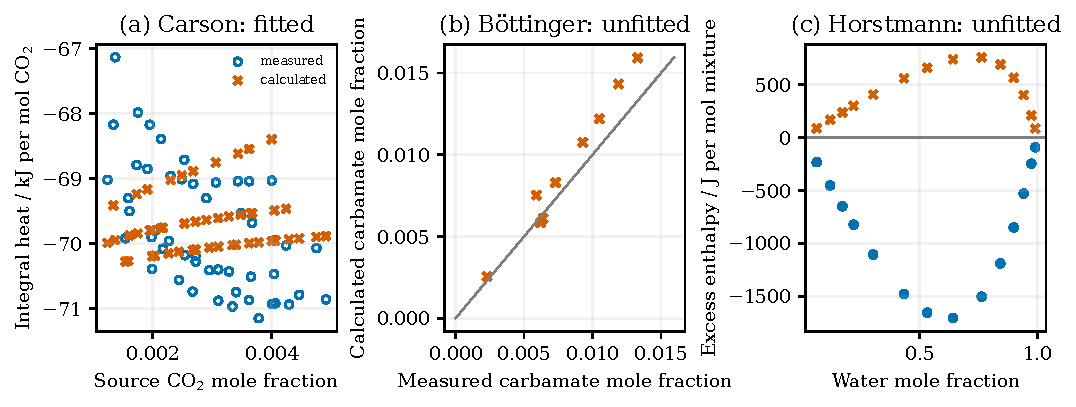
\includegraphics[width=\linewidth]{dea-properties.pdf}
\caption{DEA properties at the measured coordinates: (a) fitted Carson integral absorption heats at 298.15 K against the source \ce{CO2} mole fraction, with the source heat-release magnitude converted to negative enthalpy for exothermic absorption; (b) comparison-only carbamate mole fractions in the nine B\"ottinger states without byproduct, at assumed 2.5 MPa; (c) comparison-only water--DEA excess enthalpy at 363.15 K and 1.75 MPa. Circles are measurements and crosses calculations. The different enthalpy bases and temperatures separate the successful absorption-heat calibration from the wrong-sign mixing prediction.}
\label{fig:p2-dea-properties}
\end{figure}

% P:p2-results-other-03
DEA comparison-only pressure AARD is 41.74\,\% for Lawson Table VIII, nominally 50 wt\% but 54.5 wt\% at 77 $^{\circ}$F.
Cai binary data \cite{caiBinaryIsobaricVaporLiquid1996} give 40.82\,\% pressure AARD at 6.66 kPa, far from the fitted binary isotherm, while forty-three loaded densities at 298 K give 0.445\,\% AARD.
Those properties use different data, conditions and measurement scales (Supplementary Section~S4).
The MDEA held-out capped absorption heat at 388.71 K and 60 wt\% is $-64.491$ kJ/mol \COtwo, against $-63.3$ kJ/mol; this extrapolates the dissociation measurements and solvent concentration.
The corresponding 333.15 K, 60 wt\% capped heat could not be calculated.
PZ has no comparable reactive heat or density assessment; the four amines have not been checked equally across properties.
\FloatBarrier

\subsection{Phase behavior limits the apparent fit}\label{sec:p2-phases}
% P:p2-results-phase-opening
Small property residuals do not exclude false liquid phases: the reported PZ fit has at least forty across calibration and comparison states, and a separate fit with the Part I stability penalty still has at least three, two of which the routine search missed.
% P:p2-results-phase-02
Four false liquid splits are detected for the reported PZ fit at Hilliard rows 55, 56, 61 and 62, near 4.96--5.02 mol PZ/kg water, loading 0.77--0.83 and 313 or 333 K.
The calculated additional liquids contradict the measured liquid states despite the moderate pressure AARD.
The search examines 183 calibration states, comprising 121 NMR states and sixty-two bubble states, and finds no split at the fifty-two held-out bubble states.
Rich NMR states below their calculated bubble pressure are assessed as liquids at 1.05 times that pressure; those moved states do not demonstrate single-liquid behavior at the original assumed 0.1 MPa.

% P:p2-results-phase-kamps
Thirty-six additional false liquid splits occur at Kamps states, at 313--354 K and loading 0.96--1.64 mol \COtwo/mol PZ, with tangent-plane distances from $-0.026$ to $-0.554\,RT$.
The second liquids are rich in bicarbonate and doubly protonated PZ.
Pressures at these states belong to a single liquid that is not the stable state of this model; the split count is a lower bound.
At 1.5 times bubble pressure all four Hilliard splits persist, although the routine search misses two; all 121 NMR states pass the finite search at $T+0.5$ K, with rich states moved above bubble pressure as specified in the supplement.

% P:p2-results-phase-03
The separate PZ penalty fit does not remove the false liquid splitting.
Its routine census detects only one split, but direct tangent-plane evaluations at known split compositions show two further negative distances, $-0.0309\,RT$ and $-0.0437\,RT$, at rows 55 and 56.
The penalty fit therefore has at least three false liquid splits.
This counterexample demonstrates a missed finite search, so every split count in this paper is a lower bound, and the absence of detected instability, here and for the penalized MEA fit of Part I \cite[Sect.~4.5]{PolleyPartI}, does not prove stability.

% P:p2-results-phase-01
The MDEA searches cover 775 calculated states, some repeating a physical state; none detects an additional liquid, 37 detect a gas-like phase, and none is ambiguous or unresolved.
Seven source states above the shared R2 interval are excluded, and there is no phase evidence at 394.94--395.00 K.
AMP has no detected liquid, gas, ambiguous or unresolved outcome at the fifty-one Kundu states.
Its calibration searches retain no detected liquid, ambiguous or unresolved outcome, but their gas outcomes were not stored.
DEA searches the 140 fitted and held-out states without detecting an additional phase or an unresolved result.


% Generator: docs/scientific/latex/scripts/part2_displays.py; no model evaluation.
% Input: analyses/amp_transfer/inputs/kundu/current-declarations.toml SHA256 3085081adcf6b1d5e797a49ae6b96037cc1b5bc5191f45cff699d8546d774c55
% Input: analyses/amp_transfer/inputs/redesign/refit-306-floor-coordinates.json SHA256 b8671b1abbca5c7a406147dfad2359f1c1666887fab0b4eb67e489fc80abbe99
% Input: analyses/amp_transfer/inputs/redesign/refit-306-floor-endpoint.json SHA256 6d26e1e15c89217c7e29ce1d0772aa44285158071fdf4cc1bd0f6e7fb8fb2107
% Input: analyses/amp_transfer/notebook.qmd SHA256 a46134ecc164b9304778c6d809851a64a128dd91f932e6b898da3ce04bc9fd62
% Input: analyses/amp_transfer/results/kundu/summary.json SHA256 814f2ce5a28047c470bbcab59aadf13984e7ae034b55a4239b8e5b3058d0b55e
% Input: analyses/amp_transfer/results/refit-306/kundu-pressures.csv SHA256 561d08cf41e18d6ac277ee5e2dd207904a8885274d8d45739a0ec3f56d851cdb
% Input: analyses/amp_transfer/results/refit-306/refit-306-floor-fit.json SHA256 d7ee97cb1550d2a6969de406f09048dd4326f025a79523b7e205a5c65439233c
% Input: analyses/amp_transfer/results/refit-306/summary.json SHA256 3912f54eb7821b08e05f902d3001493b269355bea383439cada4e33fc4b4128f
% Input: analyses/amp_transfer/results/refit-306/uncertainty/prediction-bands.csv SHA256 d65f885c32fc9b391305b7e0ac76ec9f0112435455d027391c66dcd1ba7a9ff0
% Input: analyses/amp_transfer/results/refit-306/uncertainty/ranking.csv SHA256 ce80d211f43c53c9f654ec85ebdd5a91ac779a827c5e992415954cacffcab2a6
% Input: analyses/dea_transfer/inputs/runs/B-2-coordinates.json SHA256 7402f93dd3334eae251b38df951d2fdc310a730bf0045871bb83482524e75beb
% Input: analyses/dea_transfer/inputs/runs/B-2-endpoint-declarations.toml SHA256 a0e6cd9a5a7796d892130fc71f756480465898fa28cb0fc8cd371e9f4b730b72
% Input: analyses/dea_transfer/inputs/runs/B-2-endpoint-document.json SHA256 91c2384ef9f7b2a035962aafb72d97435a18a94595c5f16c64c9e2ac18785cdd
% Input: analyses/dea_transfer/notebook.qmd SHA256 c08a11c9e055d810c4b04c5c421a3ac89cf9edea895c7eb2ce3225e22368373d
% Input: analyses/dea_transfer/results/figure-values.csv SHA256 58cbb7b6e6f825b0f4fba1ef19f5393ad469e8aa42a58ece391f3b3d7af4bf2c
% Input: analyses/dea_transfer/results/fits.json SHA256 b936638b0b1f83802809bea15c003c1bbcc229b23824ce61d48ac4123b80af48
% Input: analyses/dea_transfer/results/score.json SHA256 12aa281fa03ed5d34cabbe3a09174b49da105199b15f1b16087ffa33018fd64e
% Input: analyses/dea_transfer/results/uncertainty-307/prediction-bands.csv SHA256 b59d9515e2d86b3c76eea92e97343eb5b2e28512bf4e8dd9f69e359de593f9ed
% Input: analyses/dea_transfer/results/uncertainty-307/ranking.csv SHA256 14ec3184971afe521ae4be0f1d636acd3a47067df1a01feb6068d75cf63cf155
% Input: analyses/mdea_mea_workflow/notebook.qmd SHA256 55831c2a23404765f14fbcbeb2c83eb64b7245a10730ad9ad9329b85aa1c2533
% Input: analyses/mdea_mea_workflow/results/refit-298/B1-endpoint/endpoint.json SHA256 2a5341be176829d087133a1467828f762a655f92a586eb1062a5719a58142d9d
% Input: analyses/mdea_mea_workflow/results/refit-298/B1-endpoint/fitted-replay.json SHA256 6690d0b7baf4bb3f08a9437743857d965d7a4a4fd1529d4e6f8e5d234f4059e2
% Input: analyses/mdea_mea_workflow/results/refit-298/attempts.json SHA256 40e17071831a699fe380d4ac4b1b286d5d283ad434a0e704ac2803d7d22c954f
% Input: analyses/mdea_mea_workflow/results/refit-298/pressure-comparison.csv SHA256 d2cdaf4a3bc1a2b7b9b957585a6dbaec2eff15ca56c009b862dac63a2912c22c
% Input: analyses/mea_parameter_bundle/results/selected-current-best-parameters.json SHA256 f8f64820b161377a0d97d1e4ad4f6cea764cd0558dc63231d58e2096988eef97
% Input: analyses/pz_transfer/notebook.qmd SHA256 0b5d7fe8f2e9f417972f8998257cb5108325815a49eecda383e59ef740770bae
% Input: analyses/pz_transfer/results/check-states-A12-direct.json SHA256 b5d7c54a1c14c62b090776b12c8cb8c28bbfa658fa7e87d735dd778078f5d056
% Input: analyses/pz_transfer/results/check-states-A12.json SHA256 61664db83e7284fdc2aaa6961fd3fd23c99864e6fe79b192d93e2b07f25e2530
% Input: analyses/pz_transfer/results/holdout-A12.csv SHA256 89f6aabc166a2663ddf7be4cfdc20821cc3ef9ef46070535644f5cd2abb66b15
% Input: analyses/pz_transfer/results/kamps2003-A12.csv SHA256 34f8300ca39e4a25c77f1bc834d2c22198f0ace06a4dda28ecc82eacba7bfe84
% Input: analyses/pz_transfer/results/kamps2003-A12.json SHA256 bb5f044833c67ad7b9bf911c14cf5d9b7a0d6f0c894ba8a697062250708439b9
% Input: analyses/pz_transfer/results/reactive-A12-record.json SHA256 3eefe76e4599050e524b9a1a8354121caae0ca30de38613359cf7e1f9edc1329
% Input: analyses/pz_transfer/results/reactive-A12-residuals.csv SHA256 3c8855bba6dfaa8ed8c8e64f7c4a160cafb77fb1d85b6858e8d5520e1469e4e4
% Input: analyses/pz_transfer/results/reactive-A12-start2-endpoint.json SHA256 c24ff09badc642d5dd312f5dc03248f2e5fa4c93e3b1d91fa69fe42120297b9e
% Input: analyses/pz_transfer/results/speciation-reactions.json SHA256 64a51633b7d56ce75a1246fe51eb6a39a1f0db1abc7d75b16b2fe13df9c125be
% Input: analyses/pz_transfer/results/uncertainty-A12/ranking.csv SHA256 f266707b75ee505bb8a5226c79e6f30037696720f859ca7d239972e6f58c71fe
% Input: analyses/solvent_specification_mdea/B1-declarations.toml SHA256 7b5fd083d83731c74624707f6e9f92bad05265c9ed19d105b25cf99dd897a042
% Input: analyses/solvent_specification_mdea/inputs/B1-coordinates.json SHA256 0bca9af202313b2bd8325ccaa37a72f32a1b326099c957c5ebf35f630506c8be
% Input: analyses/solvent_specification_mdea/notebook.qmd SHA256 227db268f1475ce3e11e4873c68e3337bf217918fa0ce0bdc11deeb25f57ff88
% Input: analyses/solvent_specification_mdea/results/adoption-302/B1/pressure.json SHA256 b81bfeb21d211d64211a2bda07b5e07af2a897f828a750f01aac6142340a7820
% Input: analyses/solvent_specification_mdea/results/retained-statistics-320.json SHA256 64393229910bf06ba614d1345e1fd2d2f675e2aba1a3a9a7eaedcd33ffd07e81
% Input: analyses/solvent_specification_mdea/results/uncertainty-307/prediction-bands.csv SHA256 96fc9352b6f30dae38805b799344404528d6e49b3b45eaa42002daa8523ac0cd
% Input: analyses/solvent_specification_mdea/results/uncertainty-307/predictions.json SHA256 8fd82d94b500a2b8985ea9979e4ceb653fbfb781dc66a3d047ee68bdec0f46ba
% Input: analyses/solvent_specification_mdea/results/uncertainty-307/ranking.csv SHA256 16b4ed6165c0cc7bad4d938567c8f8e8d88bdddb3de4eb8b53c43b372f7c8e7e
% Input: docs/scientific/latex/references.bib SHA256 dc2b40df7e47ccd8bc493e8d407c79d79bc8a302924bbd2d5f8cdf4320759e17
% Input: docs/scientific/latex/supplement.tex SHA256 b90143f6a0711b9a7437b4845c8a5db430f8b301ff21d8f402821b105da3d5f8
\begingroup\small\setlength{\tabcolsep}{3pt}
\begin{longtable}{@{}>{\raggedright\arraybackslash}p{0.3\linewidth}>{\raggedright\arraybackslash}p{0.2\linewidth}>{\raggedright\arraybackslash}p{0.43\linewidth}@{}}
\caption{Finite phase-search results. Detected liquid-split counts are lower bounds.}\label{tab:p2-phase-searches}\\
\toprule Fit / states & Detected liquid splits & Other outcomes and omissions \\ \midrule\endfirsthead
\toprule Fit / states & Detected liquid splits & Other outcomes and omissions \\ \midrule\endhead
\bottomrule\endfoot
MDEA: 775 searched states & 0 found & 37 gas-like phases; no ambiguous or unresolved result; seven states above the R2 interval not calculated \\
AMP: 51 Kundu states & 0 found & No gas, ambiguous or unresolved result; calibration gas outcomes not stored \\
PZ: 183 calibration states & at least 4 & No ambiguous or unresolved result; three rich NMR pressures moved above bubble pressure \\
PZ: 52 held-out bubble states & 0 found & Finite search only \\
PZ: 94 Kamps bubble states & at least 36 & 56 without detected split; 2 unloaded undecided; no gas or ambiguous split \\
PZ: compressed Hilliard states & at least 4 & At 1.5 times bubble pressure; routine search misses two \\
PZ: 121 NMR states at $T+0.5$ K & 0 found & Three rich states above 0.1 MPa evaluated at 1.05 times bubble pressure \\
PZ penalty alternative & at least 3 & One found routinely; two additional splits resolved by direct distance evaluation \\
DEA: 140 fitted/held-out states & 0 found & No gas, ambiguous or unresolved result \\
\end{longtable}\endgroup


\FloatBarrier

\section{Conclusions}\label{sec:p2-conclusions}
% P:p2-conclusions-01
A frozen description of water, \COtwo and inorganic ions can accompany amine-specific fitting across MDEA, AMP, PZ and DEA, but calibration and transfer remain property- and source-dependent.
Residual loading-shape errors persist in the fitted pressures, and PZ species residuals remain large relative to their assumed measurement scales.
Shared-parameter substitutions followed by refitting demonstrate compensation: an apparently improved unfitted AMP score before refitting does not survive restoration of its calibration fit.

% P:p2-conclusions-02
MDEA's outside-fit pressure AARDs are 28.19\,\% for Xiao and 18.27\,\% for Ermatchkov, with the latter mixing measured-range and extrapolated dissociation conditions.
AMP's held-out Kundu error is 42.85\,\%, while PZ gives 21.94\,\% against held-out Ermatchkov pressures and 48.52\,\% at 393.15 K.
DEA gives 79.54 and 44.17\,\% on the held-out Seo and Hong and Lal data, despite 0.98\,\% fitted integral-heat AARD, and predicts the wrong sign of water--DEA excess enthalpy.
These unmatched errors are not an amine ranking.

% P:p2-conclusions-03
Local conditional parameter bands are much smaller than the AMP and DEA unfitted discrepancies, overlap the MDEA errors, and are limited by large PZ sensitivities.
At least four false liquid splits remain for the reported PZ fit; a separate penalty fit and direct split evaluations demonstrate that the finite phase search can miss instability.
No additional phase was detected in the specified MDEA, AMP and DEA searches, which is numerical evidence at finite states rather than proof of stability.
The extent of transfer is therefore defined by the reported calibration errors, unfitted property failures, reaction-law extrapolations and conditional uncertainty, rather than by a universal accuracy or process-use claim.

\section*{Data and code availability}
% P:p2-availability-01
Processed observations, parameter files, numerical results and presentation scripts are provided with the public electronic data at \url{https://github.com/tannerpolley/Amine-Thermodynamics}.
Presentation code reads the stored calculations without evaluating the thermodynamic model again.
Input checksums and the source of every displayed numerical result are listed in the accompanying numerical-source index.
The calculations use the compiled \texttt{epcsaft} library identified in Supplementary Section~S8; referee access arrangements and a deposit DOI remain to be supplied before submission.
Third-party measurements retain their source terms.

\section*{Acknowledgements}
% P:p2-acknowledgements-01
Calculations used the MA57 linear solver from HSL, a collection of Fortran codes for large-scale scientific computation, \url{https://www.hsl.rl.ac.uk/}.

\section*{Funding}
% P:p2-funding-01
This research received no specific grant from funding agencies in the public, commercial, or not-for-profit sectors.

\section*{Declaration of competing interest}
% P:p2-interest-01
The author declares no known competing financial interests or personal relationships that could have appeared to influence the work reported in this paper.

\section*{CRediT author statement}
% P:p2-credit-01
Tanner W. Polley: Conceptualization, methodology, software, formal analysis, investigation, data curation, writing--original draft, writing--review and editing, visualization.

\section*{Declaration of generative AI and AI-assisted technologies}
% P:p2-ai-01
OpenAI Codex and Claude were used to prepare manuscript text and assist with computational consistency and source checking.
Author review of this first draft and its scientific claims is required before submission.

\section*{Nomenclature}
% P:p2-nomenclature-01
$\alpha$: added \COtwo per total amine, mol/mol; $w_A$: unloaded amine mass fraction; $x_i,y_i$: liquid and vapor true-species mole fractions; $P$: total pressure; $p_{\COtwo}=y_{\COtwo}P$: partial pressure; $K$: equilibrium constant on the stated standard state; $C$: least-squares cost; $s$: assigned observation scale; SE: conditional standard error; AARD: average absolute relative deviation; NMR: nuclear magnetic resonance; $k_{ij}$: unlike-pair dispersion correction; $d^{\mathrm{Born}}$: Born diameter.

\FloatBarrier
\bibliographystyle{styles/model1-num-names}
\bibliography{references,part2_companion,part2_sources}
\end{document}
